\documentclass[12pt,a4paper]{report}

% Package
\usepackage[T1]{fontenc}
\usepackage[utf8]{inputenc}
\usepackage[italian]{babel}
\usepackage{graphicx}
\usepackage{geometry}
\geometry{a4paper, margin=2.5cm}
\usepackage{ltablex}
\usepackage{booktabs}
\usepackage{float}
\usepackage{titlesec}
\usepackage{enumitem}
\usepackage[table]{xcolor}
\usepackage{array}

% CARICAMENTO HYPERREF (SEMPRE PER ULTIMO)
\usepackage{hyperref}
\hypersetup{
    colorlinks=false,
    pdfborder={0 0 0},
}

\usepackage[normalem]{ulem}

% Stile per i link esterni (sottolineatura continua)
\let\oldhref\href
\renewcommand{\href}[2]{\oldhref{#1}{\uline{#2}}}
\let\oldurl\url
\renewcommand{\url}[1]{\uline{\oldurl{#1}}}

% Stile per i riferimenti interni (sottolineatura a puntini)
\let\oldref\ref
\renewcommand{\ref}[1]{\dotuline{\oldref{#1}}}
\let\oldhyperref\hyperref
\renewcommand{\hyperref}[2][]{\oldhyperref[#1]{\dotuline{#2}}}

% Contatore per i requisiti (permette link precisi nelle tabelle)
\makeatletter
\newcounter{reqcount}
\newcommand{\reqlabel}[1]{%
    \leavevmode\Hy@raisedlink{\refstepcounter{reqcount}\label{#1}}%
    \ignorespaces
}
\makeatother

% SCELTA DEL FONT
\usepackage{lmodern} % Latin Modern (versione migliorata del default LaTeX)
% \usepackage{newtxtext,newtxmath} % Times New Roman (Serif classico, molto formale)
% \usepackage{newpxtext,newpxmath} % Palatino (Serif elegante, ottimo per tesi e report)
% \usepackage[scaled]{helvet} \renewcommand{\familydefault}{\sfdefault} % Helvetica/Arial (Senza grazie)
% \usepackage[sfdefault]{roboto} % Roboto (Moderno, lineare). Se non compila, va installato 'texlive-fonts-extra'.

% Definizione Colori
\definecolor{studyColor}{HTML}{f78a88}
\definecolor{linkColor}{HTML}{4f7ca7}

% Impostazioni
\keepXColumns
\setcounter{secnumdepth}{3}
\setcounter{tocdepth}{2}

% Capitoli
\titleformat{\chapter}
    {\normalfont\Large\bfseries\color{linkColor}}{\thechapter.\ }{0pt}{\Large}
\titlespacing*{\chapter}{0pt}{-20pt}{15pt}

% Sezioni
\titleformat{\section}
    {\normalfont\large\bfseries\color{studyColor}}{\thesection.\ }{0pt}{\large}
\titlespacing*{\section}{0pt}{10pt}{10pt}

% Sottosezioni
\titleformat{\subsection}
    {\normalfont\normalsize\bfseries\color{linkColor}}{\thesubsection.\ }{0pt}{\normalsize} 
\titlespacing*{\subsection}{0pt}{8pt}{8pt}

% Sottosottosezioni
\titleformat{\subsubsection}
    {\normalfont\normalsize\bfseries\color{studyColor}}{\thesubsubsection.\ }{0pt}{\normalsize} 
\titlespacing*{\subsubsection}{0pt}{6pt}{0pt}

% Tabelle
\renewcommand{\arraystretch}{1.5}
\setlength{\tabcolsep}{10pt}
\setlength{\intextsep}{5pt}
\setlength{\LTpre}{0pt}
\setlength{\LTpost}{0pt}


% Inizio documento
\begin{document}

% Frontepagina
\begin{titlepage}
    \pagenumbering{gobble}
    \centering
    \vspace*{1cm}
    
\includegraphics[width=0.45\textwidth]{images/logo.png}\par
    \vspace{2cm}
    {\fontsize{45}{54}\selectfont\bfseries \textcolor{studyColor}{study}\textcolor{linkColor}{Link} \par}
    \vfill
    \begin{flushright}
        {\large \textbf{Gruppo 31} \quad A.A. 2025/2026 \par}
        \vspace{0.5cm}
        Matteo Gattobigio \quad 0001117104 \\
        Lucilla Lucchi \quad 0001116767 \\
        Federico Porpora \quad 0001114450 \par
    \end{flushright}
\end{titlepage}

% Abstract
\newpage
\pagenumbering{arabic}
\chapter*{Abstract}
\addcontentsline{toc}{chapter}{Abstract}
Il progetto \textbf{studyLink} è un'applicazione nata per aiutare gli studenti universitari a trovare e formare gruppi di studio dal vivo, rendendo semplicissimo l'incontro tra colleghi.

La piattaforma punta tutto sulla trasparenza: ogni studente ha un Profilo personale chiaro e visibile.
L'applicazione gestisce le sessioni di studio in modo flessibile, permettendo agli Utenti di alternarsi in due ruoli chiave:
\begin{itemize}
    \item \textbf{L'Organizzatore}, che prende l'iniziativa e crea l'Evento scegliendo la data, l'orario, il luogo d'incontro e i posti disponibili;
    \item \textbf{Il Partecipante}, che sfoglia la Bacheca e si prenota per i gruppi già avviati occupando i posti liberi.
\end{itemize}

Inoltre, per facilitare l'organizzazione, tutti gli iscritti a un Evento hanno a disposizione una Chat di gruppo dedicata. È uno spazio comodo e privato per scambiarsi appunti, materiali di studio o mettersi d'accordo sui dettagli prima di vedersi di persona.

% Indice
\newpage
\tableofcontents

% Analisi dei requisiti
\newpage
\chapter{Analisi dei requisiti}

% Raccolta dei requisiti
\section{Raccolta dei requisiti}
\begin{itemize}[leftmargin=*]
    \item Il sistema deve permettere all'Utente di registrarsi fornendo le proprie Credenziali (Email e Password). La Registrazione è permessa esclusivamente a Utenti aventi un'Email istituzionale universitaria (es. @studio.unibo.it).
    \item Ogni Utente può gestire il proprio Profilo personale, contenente nome, cognome, Corso di studi, una breve Biografia e opzionalmente un'immagine.
    \item Qualsiasi Utente autenticato può creare un nuovo Evento.
    \item L'Organizzatore, nella creazione di un Evento, deve definire:
    \begin{itemize}
        \item \textbf{Titolo:} il titolo dell'Evento deve essere chiaro e descrittivo, nel caso anche della materia che si intende studiare nell'incontro;
        \item \textbf{Data e orario:} l'Evento deve avere una data e un orario di inizio e fine ben definiti;
        \item \textbf{Indirizzo:} indicazione fisica specifica (via, nome della struttura o aula) in cui si terrà l'incontro;
        \item \textbf{Tipo di Luogo:} scegliere tra Luogo ``Pubblico'' o ``Privato'';
        \item \textbf{Numero di posti:} può essere a posti ``Limitati'' o ``Illimitati''.
    \end{itemize}
    \item Il sistema deve offrire una Bacheca globale dove l'Utente può sfogliare gli Eventi di studio creati da altri Utenti. Gli Eventi scompaiono dalla Bacheca una volta pieni.
    \item L'Utente deve poter filtrare gli Eventi in Bacheca in base alla Materia (Specifico per Esame o Generale), Tipo di Luogo (Pubblico o Privato), numero di posti (Limitato o Illimitato), data e Indirizzo.
    \item Gli utenti scelgono l'evento in base al titolo dato dall'organizzatore
    \item Un Utente può prenotarsi per un Evento esistente se sono presenti posti disponibili.
    \item Un Partecipante può annullare la propria Prenotazione fino a un'ora prima, liberando il posto per altri Utenti.
    \item L'Organizzatore può modificare i dettagli dell'Evento o cancellarlo fino all'ora precedente. In caso di modifica o cancellazione, tutti i Partecipanti ricevono una Notifica automatica.
    \item L'Organizzatore può rimuovere gli Utenti Partecipanti a sua discrezione.
    \item Alla pubblicazione di un Evento, il sistema deve generare automaticamente una Chat di gruppo privata, accessibile esclusivamente all'Organizzatore e ai Partecipanti di quello specifico Evento.
    \item Al termine dell'Evento i Partecipanti possono lasciare dei Commenti positivi o negativi.
    \item L'interfaccia Utente deve essere intuitiva e ottimizzata per l'uso in mobilità (mobile-friendly), facilitando la navigazione rapida tra Bacheca e Chat.
    \item Le informazioni del Profilo devono essere facilmente consultabili prima di unirsi a un gruppo per favorire un clima di fiducia tra colleghi.
    \item I messaggi scambiati nella Chat devono essere visibili solo ai membri del gruppo di studio corrente. I dati personali devono essere trattati in conformità con le normative vigenti (\href{https://gdpr-info.eu/}{GDPR}).
\end{itemize}

% Requisiti di sistema
\newpage
\section{Requisiti di sistema}

\subsection{Requisiti funzionali}
\begin{tabularx}{\textwidth}{|p{2cm}|X|p{3cm}|}
    \hline
    \rowcolor{studyColor} \textbf{ID} & \textbf{Requisito} & \textbf{Tipo} \\ \hline
    \endhead
    \reqlabel{R01F}R01F & La Registrazione è ammessa solo tramite Email istituzionale & Funzionale \\ \hline
    \reqlabel{R02F}R02F & Una persona può registrarsi, creando un Profilo Utente & Funzionale \\ \hline
    \reqlabel{R03F}R03F & Un Profilo Utente è accessibile tramite Mail istituzionale e Password & Funzionale \\ \hline
    \reqlabel{R04F}R04F & Un Profilo Utente ha le seguenti informazioni: nome, cognome, Corso di studi, Bio, immagine opzionale e Commenti ricevuti & Funzionale \\ \hline
    \reqlabel{R05F}R05F & Le caratteristiche di un Evento sono: titolo, Tipo di Luogo, data, orario, Indirizzo, posti disponibili & Funzionale \\ \hline
    \reqlabel{R06F}R06F & La Materia di un Evento può essere specificata o generica & Funzionale \\ \hline
    \reqlabel{R07F}R07F & Il tipo di accesso all'Evento è aperto a tutti, chiunque può scegliere di aggiungersi, posti permettendo & Funzionale \\ \hline
    \reqlabel{R08F}R08F & Il numero di posti disponibili può essere limitato o illimitato & Funzionale \\ \hline
    \reqlabel{R09F}R09F & Gli Eventi hanno due fasi: programmato e concluso & Funzionale \\ \hline
    \reqlabel{R10F}R10F & Gli Utenti visualizzano una Bacheca globale di Eventi programmati con almeno un posto disponibile & Funzionale \\ \hline
    \reqlabel{R11F}R11F & Gli Utenti possono filtrare gli Eventi dalla Bacheca per: Tipo di Luogo, Indirizzo, data, numero posti & Funzionale \\ \hline
    \reqlabel{R12F}R12F & Un Utente può prenotarsi a un Evento, diventandone Partecipante & Funzionale \\ \hline
    \reqlabel{R13F}R13F & Un Utente prima di prenotarsi a un Evento può visualizzare il Profilo Utente dei Partecipanti & Funzionale \\ \hline
    \reqlabel{R14F}R14F & Un Partecipante può annullare la Prenotazione all'Evento fino a un'ora prima dell'inizio & Funzionale \\ \hline
    \reqlabel{R15F}R15F & L'Organizzatore può modificare i dettagli dell'Evento o cancellarlo fino all'ora precedente & Funzionale \\ \hline
    \reqlabel{R16F}R16F & Ogni modifica di un Evento invia una Notifica a tutti i Partecipanti & Funzionale \\ \hline
    \reqlabel{R17F}R17F & L'Organizzatore può rimuovere i Partecipanti all'Evento a sua discrezione & Funzionale \\ \hline
    \reqlabel{R18F}R18F & Per ogni Evento è prevista una Chat di gruppo accessibile solo ai Partecipanti & Funzionale \\ \hline
    \reqlabel{R19F}R19F & Al termine dell'Evento, ciascun Partecipante può lasciare un Commento a ognuno degli altri presenti & Funzionale \\ \hline
    \reqlabel{R20F}R20F & Un Utente può richiedere l'eliminazione del proprio Profilo & Funzionale \\ \hline
\end{tabularx}

\subsection{Requisiti non funzionali}
\begin{tabularx}{\textwidth}{|p{2cm}|X|p{3cm}|}
    \hline
    \rowcolor{studyColor} \textbf{ID} & \textbf{Requisito} & \textbf{Tipo} \\ \hline
    \endhead
        \reqlabel{R01N}R01N & La piattaforma deve essere accessibile online & Non funzionale \\ \hline
        \reqlabel{R02N}R02N & Le Credenziali di un Utente sono univoche & Non funzionale \\ \hline
        \reqlabel{R03N}R03N & L'interfaccia della Bacheca deve essere essenziale ed intuitiva & Non funzionale \\ \hline
        \reqlabel{R04N}R04N & Il fuso orario usato dall'applicazione è GMT+1 & Non funzionale \\ \hline
        \reqlabel{R05N}R05N & Il formato di data e orario è gg/mm/aa e hh:mm 24h & Non funzionale \\ \hline
        \reqlabel{R06N}R06N & L'applicazione deve rispettare le norme definite nel \href{https://gdpr-info.eu/}{GDPR} & Non funzionale \\ \hline
        \reqlabel{R07N}R07N & La Bacheca globale deve essere costantemente aggiornata & Non funzionale \\ \hline
        \reqlabel{R08N}R08N & La Password scelta dall'Utente deve essere di almeno 8 caratteri e contenere almeno un numero e un carattere speciale (\#@?!\_-) & Non funzionale \\ \hline
        \reqlabel{R09N}R09N & La ricezione ed invio dei Messaggi deve essere istantanea & Non funzionale \\ \hline
\end{tabularx}

% Analisi del dominio
\newpage
\section{Analisi del dominio}

\subsection{Vocabolario}
\begin{tabularx}{\textwidth}{|p{3cm}|X|p{3.5cm}|}
    \hline
    \rowcolor{studyColor} \textbf{Voce} & \textbf{Definizione} & \textbf{Sinonimi} \\ \hline
    \endhead
    Profilo & Insieme delle informazioni personali e accademiche che rappresentano l'identità di un Utente all'interno della piattaforma & Account \\ \hline
    Registrazione & Creazione di un Profilo da parte di uno studente & \\ \hline
    Utente & Studente che ha eseguito la Registrazione & \\ \hline
    Autenticazione & Processo tramite il quale uno studente si identifica e si associa al proprio Profilo & Accesso, Login \\ \hline
    Informazioni del Profilo & Dati inseriti dall'Utente, quali nome, cognome, Email, Corso di studi, Biografia ed eventualmente un'immagine & \\ \hline
    Password & Sequenza di caratteri segreta & \\ \hline
    Credenziali & Coppia di Email e Password & \\ \hline
    Evento & Sessione di studio programmata da un Utente, caratterizzata da un titolo, un Indirizzo, un Tipo di Luogo, una data e un orario & Sessione di studio \\ \hline
    Titolo & Nome descrittivo dell'Evento & Nome \\ \hline
    Luogo Pubblico & Luogo fisico accessibile a tutti in cui si svolge un Evento (es. biblioteca, aula studio) & \\ \hline
    Luogo Privato & Luogo fisico privato in cui si svolge un Evento & \\ \hline
    Indirizzo & Indicazione fisica specifica (via, nome della struttura o aula) in cui si terrà l'incontro & Posizione, luogo \\ \hline
    Evento a posti Limitati & Tipologia di Evento che prevede un numero massimo di partecipanti & \\ \hline
    Evento a posti Illimitati & Tipologia di Evento che non prevede un numero massimo di partecipanti & \\ \hline
    Bacheca & Sezione in cui è possibile visualizzare l'elenco degli Eventi disponibili & \\ \hline
    Organizzatore & Utente che crea, gestisce, coordina ed è Partecipante a un Evento & \\ \hline
    Partecipante & Utente che sceglie di unirsi a un Evento & Iscritto \\ \hline
    Prenotazione & Iscrizione a un Evento & Partecipazione, iscrizione \\ \hline
    Filtro & Funzionalità di ricerca che permette di restringere la visualizzazione degli Eventi in Bacheca secondo criteri specifici & \\ \hline
    Commento & Valutazione espressa dai Partecipanti su un altro Partecipante & Recensione \\ \hline
    Chat & Canale di comunicazione testuale privato, creato automaticamente per ogni Evento e riservato ai suoi Partecipanti & Chat condivisa, Chat di gruppo \\ \hline
    Messaggio & Singola comunicazione testuale inviata da un Partecipante all'interno della Chat di gruppo & \\ \hline
    Notifica & Comunicazione istantanea diretta ai Partecipanti dall'applicazione all'arrivo di un Avviso & \\ \hline
    Avviso & Comunicazione inviata dall'applicazione a un Partecipante per informarlo di un nuovo Messaggio o modifica dei dettagli dell'Evento & \\ \hline
\end{tabularx}

% Analisi dei requisiti
\newpage
\section{Analisi dei requisiti}

\subsection{Modello dei casi d'uso}
L'analisi dei requisiti e del dominio hanno portato ai seguenti casi d'uso che interagiscono fra di loro come descritto nel seguente schema.

\begin{figure}[H]
    \centering
    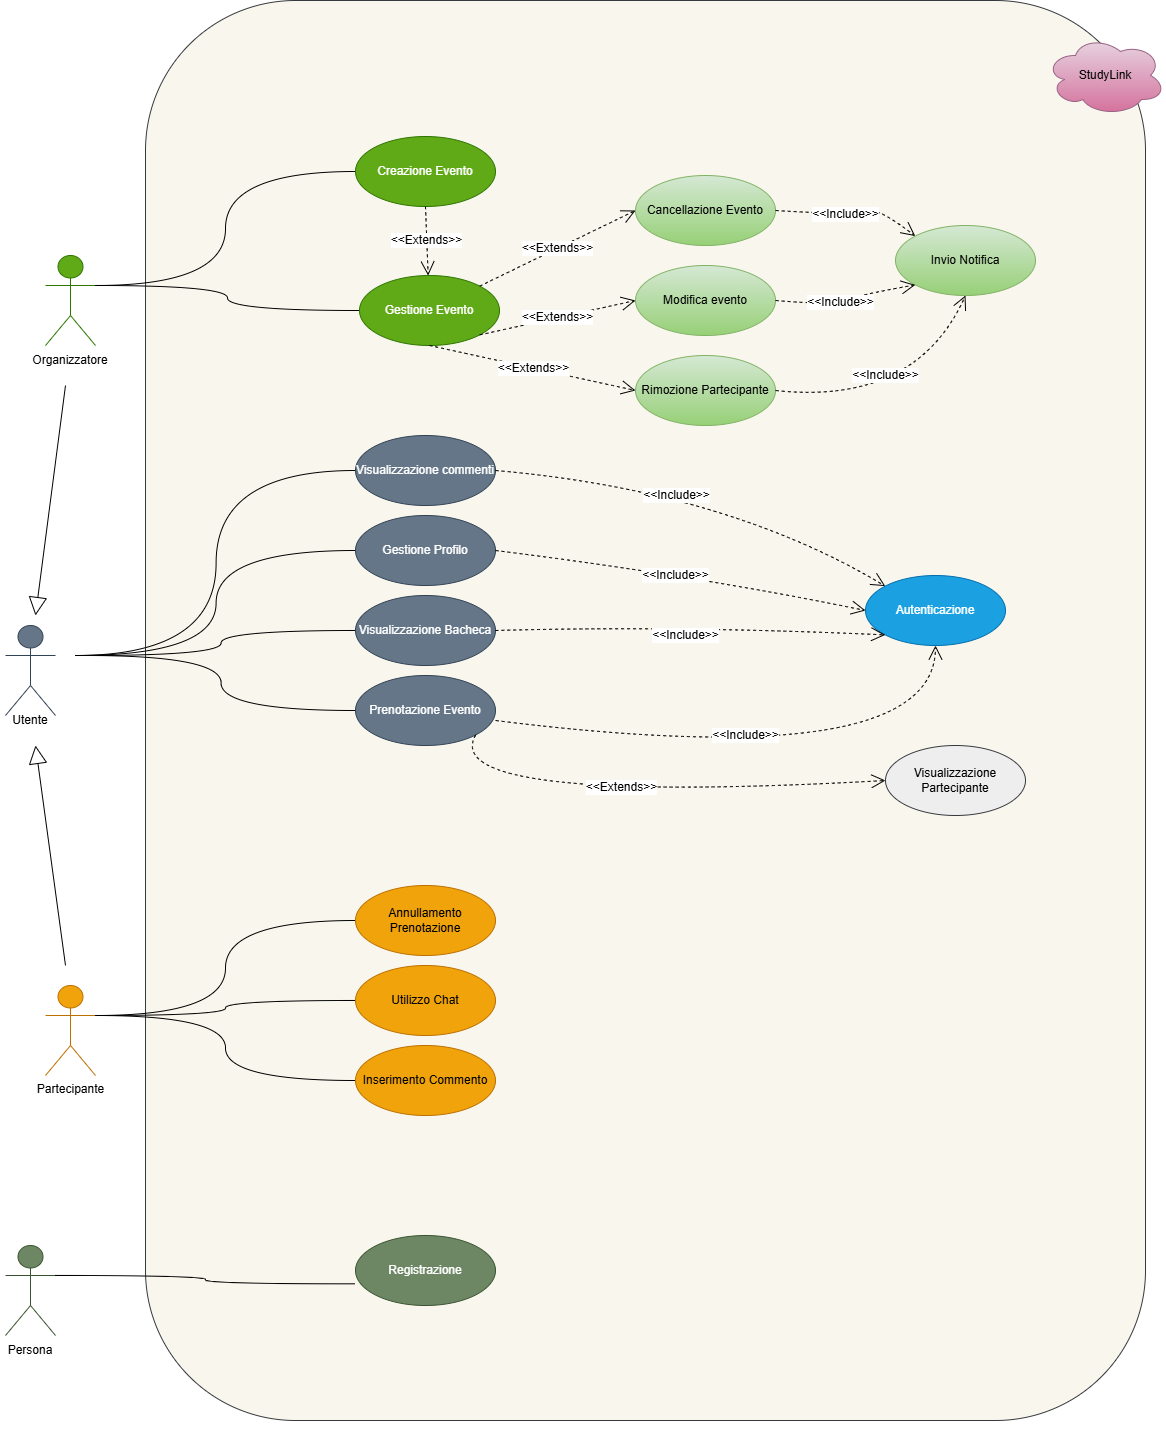
\includegraphics[width=\textwidth]{images/modello-dei-casi-d-uso.png}
\end{figure}

\newpage
\subsection{Scenari}
Di seguito sono presentati tutti gli scenari nel loro dettaglio.

\subsubsection{Registrazione}
\reqlabel{tab:Registrazione}
\begin{tabularx}{\textwidth}{|X|X|}
    \hline
    \rowcolor{studyColor} \textbf{Titolo} & \textbf{Registrazione} \\ \hline
    \endhead
    \textbf{Descrizione} & Procedura di creazione di un account Utente \\ \hline
    \textbf{Attori} & Studente \\ \hline
    \textbf{Relazioni} & \\ \hline
    \textbf{Precondizioni} & \\ \hline
    \textbf{Postcondizioni} & Il sistema memorizza il nuovo Utente \\ \hline
    \textbf{Scenario principale} &
        \begin{enumerate}[nosep, leftmargin=*]
            \item Il sistema richiede i dati per la registrazione
            \begin{itemize}[nosep, leftmargin=*]
                \item Email
                \item Password
            \end{itemize}
            \item L'attore inserisce i dati richiesti
            \item Il sistema verifica la validità delle credenziali
            \item Il sistema crea il nuovo Utente
        \end{enumerate} \\ \hline
    \textbf{Scenari alternativi} & 
        \begin{itemize}[nosep, leftmargin=*]
            \item L'Email fornita è già in uso
            \begin{enumerate}[nosep, leftmargin=*]
                \setcounter{enumi}{3}
                \item Il sistema informa l'Utente che la Email è già registrata
                \item Viene mostrata la schermata di autenticazione
            \end{enumerate}
            \item La Password non è sicura
            \begin{enumerate}[nosep, leftmargin=*]
                \setcounter{enumi}{3}
                \item Viene mostrato un messaggio di errore
                \item Lo studente può inserire una nuova Password
            \end{enumerate}
            \item La Email non è istituzionale
            \begin{enumerate}[nosep, leftmargin=*]
                \setcounter{enumi}{3}
                \item Viene mostrato un messaggio di errore
                \item Lo studente può inserire una nuova Email
            \end{enumerate}
        \end{itemize} \\ \hline
    \textbf{Requisiti non funzionali} & \hyperref[R03N]{R03N}, \hyperref[R07N]{R07N}, \hyperref[R09N]{R09N} \\ \hline
    \textbf{Punti aperti} & \\ \hline
\end{tabularx}

\newpage
\subsubsection{Autenticazione}
\reqlabel{tab:Autenticazione}
\begin{tabularx}{\textwidth}{|X|X|}
    \hline
    \rowcolor{studyColor} \textbf{Titolo} & \textbf{Autenticazione} \\ \hline
    \endhead
    \textbf{Descrizione} & L'Utente inserisce le proprie Credenziali e si autentica sulla piattaforma \\ \hline
    \textbf{Attori} & Utente \\ \hline
    \textbf{Relazioni} &
        \begin{itemize}[nosep, leftmargin=*]
            \item \hyperref[tab:Visualizzazione Commenti]{Visualizzazione Commenti}
            \item \hyperref[tab:Gestione Profilo]{Gestione Profilo}
            \item \hyperref[tab:Visualizzazione Bacheca]{Visualizzazione Bacheca}
            \item \hyperref[tab:Prenotazione Evento]{Prenotazione Evento}
            \item \hyperref[tab:Creazione Evento]{Creazione Evento}
            \item \hyperref[tab:Gestione Evento]{Gestione Evento}
            \item \hyperref[tab:Rimozione Partecipante]{Rimozione Partecipante}
            \item \hyperref[tab:Annullamento Prenotazione]{Annullamento Prenotazione}
            \item \hyperref[tab:Utilizzo Chat]{Utilizzo Chat}
            \item \hyperref[tab:Inserimento Commento]{Inserimento Commento}
        \end{itemize} \\ \hline
    \textbf{Precondizioni} & L'Utente è registrato nel sistema \\ \hline
    \textbf{Postcondizioni} & L'Utente è autenticato nel sistema \\ \hline
    \textbf{Scenario principale} &
        \begin{enumerate}[nosep, leftmargin=*]
            \item Il sistema richiede l'inserimento delle Credenziali di accesso
            \item L'Utente inserisce le proprie credenziali
            \item Il sistema verifica che le credenziali appartengano a un Utente
            \item L'Utente è autenticato nel sistema
        \end{enumerate} \\ \hline
    \textbf{Scenari alternativi} & 
        \begin{itemize}[nosep, leftmargin=*] %, before=\vspace{-0.5\baselineskip}, after=\vspace{-0.8\baselineskip}
            \item Le Credenziali sono errate
            \begin{enumerate}[nosep, leftmargin=*]
                \setcounter{enumi}{3}
                \item Viene mostrato un messaggio di errore
                \item L'Utente può reinserire le Credenziali
            \end{enumerate}
        \end{itemize} \\ \hline
    \textbf{Requisiti non funzionali} & \hyperref[R03N]{R03N}, \hyperref[R07N]{R07N}, \hyperref[R09N]{R09N} \\ \hline
    \textbf{Punti aperti} & \\ \hline
\end{tabularx}

\newpage
\subsubsection{Gestione profilo}
\reqlabel{tab:GestioneProfilo}
\begin{tabularx}{\textwidth}{|X|X|}
    \hline
    \rowcolor{studyColor} \textbf{Titolo} & \textbf{Gestione profilo} \\ \hline
    \endhead
    \textbf{Descrizione} & Inserimento, modifica o eliminazione di dati specifici dell'Utente \\ \hline
    \textbf{Attori} & Utente \\ \hline
    \textbf{Relazioni} &
        \begin{itemize}[nosep, leftmargin=*]
            \item \hyperref[tab:Autenticazione]{Autenticazione}
        \end{itemize} \\ \hline
    \textbf{Precondizioni} & \\ \hline
    \textbf{Postcondizioni} & Le modifiche del profilo sono memorizzate nel sistema \\ \hline
    \textbf{Scenario principale} &
        \begin{enumerate}[nosep, leftmargin=*]
            \item \hyperref[tab:Autenticazione]{Autenticazione}
            \item Il sistema mostra le funzionalità disponibili:
            \begin{enumerate}[nosep, leftmargin=*]
                \item Inserire e modificare i propri dati come:
                \begin{itemize}[nosep, leftmargin=*]
                    \item Nome
                    \item Cognome
                    \item Password
                    \item Corso di studi
                    \item Biografia
                    \item Immagine
                \end{itemize}
                \item Eliminare l'account dal sistema
            \end{enumerate}
            \item Il sistema apporta le modifiche effettuate
        \end{enumerate} \\ \hline
    \textbf{Scenari alternativi} & 
        \begin{itemize}[nosep, leftmargin=*]
            \item La Password non è sicura
            \begin{enumerate}[nosep, leftmargin=*]
                \setcounter{enumi}{2}
                \item Viene mostrato un messaggio di errore
                \item L'Utente può inserire una nuova Password
            \end{enumerate}
            \item La Biografia è troppo lunga
            \begin{enumerate}[nosep, leftmargin=*]
                \setcounter{enumi}{2}
                \item Viene mostrato un messaggio di errore
                \item L'Utente può inserire una nuova Biografia
            \end{enumerate}
            \item L'Immagine è troppo grande
            \begin{enumerate}[nosep, leftmargin=*]
                \setcounter{enumi}{2}
                \item Viene mostrato un messaggio di errore
                \item L'Utente può inserire una nuova Immagine
            \end{enumerate}
        \end{itemize} \\ \hline
    \textbf{Requisiti non funzionali} & \hyperref[R02N]{R02N}, \hyperref[R07N]{R07N}, \hyperref[R09N]{R09N} \\ \hline
    \textbf{Punti aperti} & \\ \hline
\end{tabularx}

\newpage
\subsubsection{Creazione Evento}
\reqlabel{tab:Creazione Evento}
\begin{tabularx}{\textwidth}{|X|X|}
    \hline
    \rowcolor{studyColor} \textbf{Titolo} & \textbf{Creazione Evento} \\ \hline
    \endhead
    \textbf{Descrizione} & L'Organizzatore inserisce i dettagli necessari per programmare una nuova sessione di studio \\ \hline
    \textbf{Attori} & Utente \\ \hline
    \textbf{Relazioni} &
        \begin{itemize}[nosep, leftmargin=*]
            \item \hyperref[tab:Autenticazione]{Autenticazione}
        \end{itemize} \\ \hline
    \textbf{Precondizioni} & \\ \hline
    \textbf{Postcondizioni} & Il sistema memorizza le modifiche effettuate e l'Utente diventa Organizzatore e Partecipante all'Evento \\ \hline
    \textbf{Scenario principale} &
        \begin{enumerate}[nosep, leftmargin=*]
            \item \hyperref[tab:Autenticazione]{Autenticazione}
            \item Il sistema mostra la possibilità di creare un Evento
            \item Il sistema mostra i dati relativi all'Evento:
                \begin{itemize}[nosep, leftmargin=*]
                    \item Titolo dell'Evento
                    \item Numero di partecipanti (posti Limitati o Illimitati)
                    \item Tipo di Luogo
                    \item Indirizzo
                    \item Data
                    \item Orario
                \end{itemize}
            \item Il sistema verifica la presenza e validità dei dati
            \item Il sistema apporta le modifiche effettuate
        \end{enumerate} \\ \hline
    \textbf{Scenari alternativi} & 
        \begin{itemize}[nosep, leftmargin=*]
            \item Dei campi sono stati omessi
            \begin{enumerate}[nosep, leftmargin=*]
                \setcounter{enumi}{4}
                \item Viene mostrato un messaggio che indica i campi mancanti
                \item L'Utente può inserire nuovamente i dati mancanti
            \end{enumerate}
            \item La data scelta è antecedente alla data corrente
            \begin{enumerate}[nosep, leftmargin=*]
                \setcounter{enumi}{4}
                \item Viene mostrato un messaggio di errore
                \item L'Utente può inserire una nuova data
            \end{enumerate}
            \item Il numero di posti inseriti non è valido
            \begin{enumerate}[nosep, leftmargin=*]
                \setcounter{enumi}{4}
                \item Viene mostrato un messaggio di errore
                \item L'Utente può inserire un numero di partecipanti valido
            \end{enumerate}
            \item L'Indirizzo o il Tipo di Luogo non sono validi o non esistenti
            \begin{enumerate}[nosep, leftmargin=*]
                \setcounter{enumi}{4}
                \item Viene mostrato un messaggio di errore
                \item L'Utente può inserire un nuovo Indirizzo
            \end{enumerate}
        \end{itemize} \\ \hline
    \textbf{Requisiti non funzionali} & \hyperref[R04N]{R04N}, \hyperref[R05N]{R05N}, \hyperref[R07N]{R07N} \\ \hline
    \textbf{Punti aperti} & \\ \hline
\end{tabularx}

\newpage
\subsubsection{Gestione Evento}
\reqlabel{tab:Gestione Evento}
\begin{tabularx}{\textwidth}{|X|X|}
    \hline
    \rowcolor{studyColor} \textbf{Titolo} & \textbf{Gestione Evento} \\ \hline
    \endhead
    \textbf{Descrizione} & L'Organizzatore modifica i dettagli dell'Evento \\ \hline
    \textbf{Attori} & Organizzatore \\ \hline
    \textbf{Relazioni} &
        \begin{itemize}[nosep, leftmargin=*]
            \item \hyperref[tab:Autenticazione]{Autenticazione}
        \end{itemize} \\ \hline
    \textbf{Precondizioni} & L'Evento deve esistere \\ \hline
    \textbf{Postcondizioni} & Le modifiche dell'Evento sono memorizzate nel sistema \\ \hline
    \textbf{Scenario principale} &
        \begin{enumerate}[nosep, leftmargin=*]
            \item \hyperref[tab:Autenticazione]{Autenticazione}
            \item Il sistema mostra le funzionalità disponibili:
            \begin{enumerate}[nosep, leftmargin=*]
                \item Modificare i dettagli relativi all'Evento creato:
                \begin{itemize}[nosep, leftmargin=*]
                    \item Titolo dell'Evento
                    \item Numero di Partecipanti (posti Limitati o Illimitati)
                    \item Tipo di Luogo
                    \item Indirizzo
                    \item Data
                    \item Orario
                \end{itemize}
                \item Eliminare l'Evento
            \end{enumerate}
            \item Il sistema notifica i Partecipanti delle modifiche
            \item Il sistema apporta le modifiche effettuate
        \end{enumerate} \\ \hline
    \textbf{Scenari alternativi} & 
        \begin{itemize}[nosep, leftmargin=*]
            \item Il Numero di Partecipanti inserito è minore del numero di Partecipanti attuali
            \begin{enumerate}[nosep, leftmargin=*]
                \setcounter{enumi}{2}
                \item Viene mostrato un messaggio di errore
                \item L'Organizzatore può inserire un numero di partecipanti valido
            \end{enumerate}
            \item Dei campi sono stati omessi
            \begin{enumerate}[nosep, leftmargin=*]
                \setcounter{enumi}{2}
                \item Viene mostrato un messaggio che indica i campi mancanti
                \item L'Utente può inserire nuovamente i dati mancanti
            \end{enumerate}
            \item La data scelta è antecedente alla data corrente
            \begin{enumerate}[nosep, leftmargin=*]
                \setcounter{enumi}{2}
                \item Viene mostrato un messaggio di errore
                \item L'Utente può inserire una nuova data
            \end{enumerate}
            \item Il numero di posti inseriti non è valido
            \begin{enumerate}[nosep, leftmargin=*]
                \setcounter{enumi}{2}
                \item Viene mostrato un messaggio di errore
                \item L'Utente può inserire un numero di partecipanti valido
            \end{enumerate}
            \item L'Indirizzo o il Tipo di Luogo non sono validi o non esistenti
            \begin{enumerate}[nosep, leftmargin=*]
                \setcounter{enumi}{2}
                \item Viene mostrato un messaggio di errore
                \item L'Utente può inserire un nuovo Indirizzo
            \end{enumerate}
        \end{itemize} \\ \hline
    \textbf{Requisiti non funzionali} & \hyperref[R03N]{R03N}, \hyperref[R07N]{R07N}, \hyperref[R09N]{R09N} \\ \hline
    \textbf{Punti aperti} & \\ \hline
\end{tabularx}

\newpage
\subsubsection{Rimozione Partecipante}
\reqlabel{tab:Rimozione Partecipante}
\begin{tabularx}{\textwidth}{|X|X|}
    \hline
    \rowcolor{studyColor} \textbf{Titolo} & \textbf{Rimozione Partecipante} \\ \hline
    \endhead
    \textbf{Descrizione} & L'Organizzatore rimuove un Partecipante dall'Evento \\ \hline
    \textbf{Attori} & Organizzatore \\ \hline
    \textbf{Relazioni} &
        \begin{itemize}[nosep, leftmargin=*]
            \item \hyperref[tab:Autenticazione]{Autenticazione}
            \item \hyperref[tab:Gestione Evento]{Gestione Evento}
        \end{itemize} \\ \hline
    \textbf{Precondizioni} & L'Evento deve esistere \\ \hline
    \textbf{Postcondizioni} & Le modifiche dell'Evento sono memorizzate nel sistema \\ \hline
    \textbf{Scenario principale} &
        \begin{enumerate}[nosep, leftmargin=*]
            \item \hyperref[tab:Autenticazione]{Autenticazione}
            \item Il sistema mostra all'Organizzatore la possibilità di rimuovere un Partecipante
            \item L'Organizzatore seleziona il Partecipante da rimuovere
            \item Il sistema aggiorna l'Evento rimuovendo il Partecipante
            \item Il sistema notifica il Partecipante della rimozione dall'Evento
            \item Il sistema apporta le modifiche effettuate
        \end{enumerate} \\ \hline
    \textbf{Scenari alternativi} \\ \hline
    \textbf{Requisiti non funzionali} & \hyperref[R03N]{R03N}, \hyperref[R07N]{R07N}, \hyperref[R09N]{R09N} \\ \hline
    \textbf{Punti aperti} & \\ \hline
\end{tabularx}

\newpage
\subsubsection{Visualizzazione Bacheca}
\reqlabel{tab:Visualizzazione Bacheca}
\begin{tabularx}{\textwidth}{|X|X|}
    \hline
    \rowcolor{studyColor} \textbf{Titolo} & \textbf{Visualizzazione Bacheca} \\ \hline
    \endhead
    \textbf{Descrizione} & L'Utente visualizza tutti gli Eventi disponibili con la possibilità di applicare Filtri \\ \hline
    \textbf{Attori} & Utente \\ \hline
    \textbf{Relazioni} & 
        \begin{itemize}[nosep, leftmargin=*]
            \item \hyperref[tab:Autenticazione]{Autenticazione}
        \end{itemize} \\ \hline
    \textbf{Precondizioni} & \\ \hline
    \textbf{Postcondizioni} & \\ \hline
    \textbf{Scenario principale} &
        \begin{enumerate}[nosep, leftmargin=*]
            \item \hyperref[tab:Autenticazione]{Autenticazione}
            \item Il sistema mostra all'Utente la Bacheca degli Eventi
            \item Il sistema mostra la possibilità di applicare i seguenti Filtri:
                \begin{itemize}[nosep, leftmargin=*]
                    \item Data
                    \item Indirizzo
                    \item Tipo di Luogo
                    \item Numero di Partecipanti
                \end{itemize}
                \item L'Utente inserisce le condizioni del Filtro
                \item Il sistema mostra gli Eventi che rispettano le condizioni applicate
        \end{enumerate} \\ \hline
    \textbf{Scenari alternativi} & \\ \hline
    \textbf{Requisiti non funzionali} & \hyperref[R03N]{R03N}, \hyperref[R07N]{R07N}, \hyperref[R09N]{R09N} \\ \hline
    \textbf{Punti aperti} & \\ \hline
\end{tabularx}

\newpage
\subsubsection{Prenotazione Evento}
\reqlabel{tab:Prenotazione Evento}
\begin{tabularx}{\textwidth}{|X|X|}
    \hline
    \rowcolor{studyColor} \textbf{Titolo} & \textbf{Prenotazione Evento} \\ \hline
    \endhead
    \textbf{Descrizione} & Permette all'Utente di prenotare un Evento dalla Bacheca \\ \hline
    \textbf{Attori} & Utente \\ \hline
    \textbf{Relazioni} &
        \begin{itemize}[nosep, leftmargin=*]
            \item \hyperref[tab:Autenticazione]{Autenticazione}
            \item \hyperref[tab:Visualizzazione Bacheca]{Visualizzazione Bacheca}
        \end{itemize} \\ \hline
    \textbf{Precondizioni} & \\ \hline
    \textbf{Postcondizioni} & L'Utente diventa Partecipante dell'Evento \\ \hline
    \textbf{Scenario principale} &
        \begin{enumerate}[nosep, leftmargin=*]
            \item \hyperref[tab:Autenticazione]{Autenticazione}
            \item L'Utente seleziona un Evento dalla Bacheca
            \item Il sistema mostra i dettagli dell'Evento e i suoi Partecipanti
            \item L'Utente conferma la sua prenotazione all'Evento
            \item Il sistema apporta le modifiche effettuate
        \end{enumerate} \\ \hline
    \textbf{Scenari alternativi} & \\ \hline
    \textbf{Requisiti non funzionali} & \hyperref[R03N]{R03N}, \hyperref[R07N]{R07N}, \hyperref[R09N]{R09N} \\ \hline
    \textbf{Punti aperti} & \\ \hline
\end{tabularx}

\newpage
\subsubsection{Visualizzazione Partecipante}
\reqlabel{tab:Visualizzazione Partecipante}
\begin{tabularx}{\textwidth}{|X|X|}
    \hline
    \rowcolor{studyColor} \textbf{Titolo} & \textbf{Visualizzazione Partecipante} \\ \hline
    \endhead
    \textbf{Descrizione} & Permette agli Utenti di visualizzare i dettagli e i commenti dei Partecipanti ad un Evento \\ \hline
    \textbf{Attori} & Utente \\ \hline
    \textbf{Relazioni} & 
        \begin{itemize}[nosep, leftmargin=*]
            \item \hyperref[tab:Autenticazione]{Autenticazione}
            \item \hyperref[tab:Visualizzazione Bacheca]{Visualizzazione Bacheca}
        \end{itemize} \\ \hline
    \textbf{Precondizioni} & \\ \hline
    \textbf{Postcondizioni} & \\ \hline
    \textbf{Scenario principale} &
        \begin{enumerate}[nosep, leftmargin=*]
            \item \hyperref[tab:Autenticazione]{Autenticazione}
            \item L'Utente seleziona un Evento dalla Bacheca
            \item Il sistema mostra i dettagli dell'Evento e i suoi Partecipanti
            \item Il sistema mostra all'Utente la possibilità di visualizzare i dettagli ed i commenti dei Partecipanti
        \end{enumerate} \\ \hline
    \textbf{Scenari alternativi} & \\ \hline
    \textbf{Requisiti non funzionali} & \hyperref[R03N]{R03N}, \hyperref[R07N]{R07N}, \hyperref[R09N]{R09N} \\ \hline
    \textbf{Punti aperti} & \\ \hline
\end{tabularx}

\newpage
\subsubsection{Visualizzazione Commenti}
\reqlabel{tab:Visualizzazione Commenti}
\begin{tabularx}{\textwidth}{|X|X|}
    \hline
    \rowcolor{studyColor} \textbf{Titolo} & \textbf{Visualizzazione Commenti} \\ \hline
    \endhead
    \textbf{Descrizione} & Permette all'Utente di visualizzare i commenti presenti sul suo Profilo \\ \hline
    \textbf{Attori} & Utente \\ \hline
    \textbf{Relazioni} & 
        \begin{itemize}[nosep, leftmargin=*]
            \item \hyperref[tab:Autenticazione]{Autenticazione}
        \end{itemize} \\ \hline
    \textbf{Precondizioni} & \\ \hline
    \textbf{Postcondizioni} & \\ \hline
    \textbf{Scenario principale} &
        \begin{enumerate}[nosep, leftmargin=*]
            \item \hyperref[tab:Autenticazione]{Autenticazione}
            \item Il sistema mostra all'Utente la possibilità di visualizzare i commenti che gli altri Utenti hanno lasciato su di lui
        \end{enumerate} \\ \hline
    \textbf{Scenari alternativi} & \\ \hline
    \textbf{Requisiti non funzionali} & \hyperref[R03N]{R03N}, \hyperref[R07N]{R07N}, \hyperref[R09N]{R09N} \\ \hline
    \textbf{Punti aperti} & \\ \hline
\end{tabularx}

\newpage
\subsubsection{Annullamento Prenotazione}
\reqlabel{tab:Annullamento Prenotazione}
\begin{tabularx}{\textwidth}{|X|X|}
    \hline
    \rowcolor{studyColor} \textbf{Titolo} & \textbf{Annullamento Prenotazione} \\ \hline
    \endhead
    \textbf{Descrizione} & L'Utente annulla una prenotazione effettuata in precedenza \\ \hline
    \textbf{Attori} & Utente \\ \hline
    \textbf{Relazioni} & 
        \begin{itemize}[nosep, leftmargin=*]
            \item \hyperref[tab:Autenticazione]{Autenticazione}
        \end{itemize} \\ \hline
    \textbf{Precondizioni} & L'Utente deve essere iscritto ad un Evento \\ \hline
    \textbf{Postcondizioni} & La Prenotazione all'Evento viene annullata \\ \hline
    \textbf{Scenario principale} &
        \begin{enumerate}[nosep, leftmargin=*]
            \item \hyperref[tab:Autenticazione]{Autenticazione}
            \item Il sistema mostra all'Utente la lista delle Prenotazioni attive
            \item L'Utente seleziona la Prenotazione da annullare
            \item Il sistema apporta le modifiche effettuate
        \end{enumerate} \\ \hline
    \textbf{Scenari alternativi} & \\ \hline
    \textbf{Requisiti non funzionali} & \hyperref[R03N]{R03N}, \hyperref[R07N]{R07N}, \hyperref[R09N]{R09N} \\ \hline
    \textbf{Punti aperti} & \\ \hline
\end{tabularx}

\newpage
\subsubsection{Utilizzo Chat}
\reqlabel{tab:Utilizzo Chat}
\begin{tabularx}{\textwidth}{|X|X|}
    \hline
    \rowcolor{studyColor} \textbf{Titolo} & \textbf{Utilizzo Chat} \\ \hline
    \endhead
    \textbf{Descrizione} & Permette al Partecipante di comunicare con gli altri Partecipanti ad un Evento tramite messaggi \\ \hline
    \textbf{Attori} & Partecipante \\ \hline
    \textbf{Relazioni} & 
        \begin{itemize}[nosep, leftmargin=*]
            \item \hyperref[tab:Autenticazione]{Autenticazione}
            \item \hyperref[tab:Prenotazione Evento]{Prenotazione Evento}
        \end{itemize} \\ \hline
    \textbf{Precondizioni} & Il Partecipante deve essere iscritto all'Evento \\ \hline
    \textbf{Postcondizioni} & La comunicazione avviene con successo tra tutti i Partecipanti \\ \hline
    \textbf{Scenario principale} &
        \begin{enumerate}[nosep, leftmargin=*]
            \item \hyperref[tab:Autenticazione]{Autenticazione}
            \item Il Partecipante seleziona l'Evento
            \item Il sistema mostra la chat dell'Evento
            \item Avviene uno scambio di messaggi tra i Partecipanti
        \end{enumerate} \\ \hline
    \textbf{Scenari alternativi} & \\ \hline
    \textbf{Requisiti non funzionali} & \hyperref[R03N]{R03N}, \hyperref[R07N]{R07N}, \hyperref[R09N]{R09N} \\ \hline
    \textbf{Punti aperti} & \\ \hline
\end{tabularx}

\newpage
\subsubsection{Inserimento Commento}
\reqlabel{tab:Inserimento Commento}
\begin{tabularx}{\textwidth}{|X|X|}
    \hline
    \rowcolor{studyColor} \textbf{Titolo} & \textbf{Inserimento Commento} \\ \hline
    \endhead
    \textbf{Descrizione} & Alla chiusura di un Evento, un Partecipante inserisce un commento nel profilo di un altro Partecipante \\ \hline
    \textbf{Attori} & Partecipante \\ \hline
    \textbf{Relazioni} & 
        \begin{itemize}[nosep, leftmargin=*]
            \item \hyperref[tab:Autenticazione]{Autenticazione}
            \item \hyperref[tab:Prenotazione Evento]{Prenotazione Evento}
        \end{itemize} \\ \hline
    \textbf{Precondizioni} & Il Partecipante deve essere iscritto all'Evento \\ \hline
    \textbf{Postcondizioni} & Il commento viene salvato nel profilo del Partecipante destinatario \\ \hline
    \textbf{Scenario principale} &
        \begin{enumerate}[nosep, leftmargin=*]
            \item \hyperref[tab:Autenticazione]{Autenticazione}
            \item Il Partecipante seleziona l'Evento passato
            \item Il sistema mostra la lista dei Partecipanti all'Evento
            \item Il Partecipante seleziona il Partecipante destinatario
            \item Il Partecipante aggiunge un commento per il Partecipante selezionato
        \end{enumerate} \\ \hline
    \textbf{Scenari alternativi} & \\ \hline
    \textbf{Requisiti non funzionali} & \hyperref[R03N]{R03N}, \hyperref[R07N]{R07N}, \hyperref[R09N]{R09N} \\ \hline
    \textbf{Punti aperti} & \\ \hline
\end{tabularx}

% Analisi del Rischio
\newpage
\section{Analisi del Rischio}

\subsection{Tabella valutazione dei beni}
\begin{tabularx}{\textwidth}{|X|X|X|}
    \hline
    \rowcolor{studyColor} \textbf{Bene} & \textbf{Valore} & \textbf{Esposizione} \\ \hline
    \endhead
    Sistema Informativo & \textbf{Alto.} L'infrastruttura è fondamentale per garantire l'accesso alla Bacheca, la gestione delle Prenotazioni e le Chat in tempo
        & \textbf{Alta.} L'indisponibilità di un sistema causerebbe l'interruzione del servizio e l'impossibilità per gli studenti di incontrarsi \\ \hline
    Dati Profilo Utente e Credenziali & \textbf{Alto.} Contiene dati strettamente personali tutelati dal (\href{https://gdpr-info.eu/}{GDPR}): Credenziali e informazioni fornite dall'Utente 
        & \textbf{Alta.} In caso di furto c'è il rischio di gravi violazioni della privacy \\ \hline
    Dati Eventi e Prenotazioni & \textbf{Molto Alto.} Questi dati rivelano l'indirizzo fisico esatto, la data e l'orario in cui un gruppo specifico di studenti si troverà
        & \textbf{Molto Alta.} L'esposizione non autorizzata di questi dati comporta rischi per la sicurezza degli studenti \\ \hline
    Contenuto Chat di Gruppo & \textbf{Medio.} Le chat sono canali privati accessibili esclusivamente dai Partecipanti all'Evento 
        & \textbf{Media.} L'intercettazione dei messaggi comprometterebbe la riservatezza dell'incontro\\ \hline
\end{tabularx}

\subsection{Tabella minacce e controlli}
\begin{tabularx}{\textwidth}{|X|X|X|X|}
    \hline
    \rowcolor{studyColor} \textbf{Minaccia} & \textbf{Probabilità} & \textbf{Controllo} & \textbf{Rischio} \\ \hline
    \endhead
    Furto Credenziali Utente & \textbf{Media.} La Mail istituzionale è nota, le password devono essere indovinate & Imposizione di requisiti di sicurezza sulle Password limitazioni di tentativi di accesso
        & \textbf{Costo Medio-basso.} L'Utente è obbligato a memorizzare una password più difficile \\ \hline
    Intercettazione delle comunicazioni & \textbf{Alta.} L'app viene usata in mobilità spesso su reti wi-fi universitarie o pubbliche non sempre sicure & Cifratura delle comunicazioni
        & \textbf{Costo basso.} Le tecnologie per la cifratura del traffico web sono gratuite e facilmente integrabili \\ \hline
    Denial of Service & \textbf{Alta.} Essendo un servizio esposto su rete pubblica, chiunque può tentare un attacco DoS & Progettazione infrastruttura adeguata 
        & \textbf{Costo basso.} Prevenzione effettuabile attraverso la limitazione di richieste per uno stesso Utente \\ \hline
    Accesso non autorizzato alle Chat private e Dati Evento & \textbf{Media.} Un Utente potrebbe tentare di leggere le Chat di Gruppi a cui non è iscritto manipolando le chiamate al Server
        & Severo controllo degli accessi, verifica che l'Utente richiedente della Chat partecipi effettivamente all'evento
        & \textbf{Costo basso.} Richiede attenzione nella scrittura del codice, verificare sempre il ruolo dell'Utente \\ \hline
    Manomissione del Database & \textbf{Bassa.} Difficile a meno di gravi falle nel codice & Mantenimento di un file di Log inalterabile e separato per le operazioni sensibili
        & \textbf{Costo medio.} Richiede un'infrastruttura ben progettata e la creazione del componente di Log \\ \hline
\end{tabularx}

\subsection{Analisi tecnologica della sicurezza}
\begin{tabularx}{\textwidth}{|X|X|}
    \hline
    \rowcolor{studyColor} \textbf{Tecnologia} & \textbf{Vulnerabilità} \\ \hline
    \endhead
    Autenticazione tramite Credenziali & \begin{itemize}[nosep, leftmargin=*]
                    \item Password banali;
                    \item Password cracking;
                    \item Social Engineering;
                    \item Negligenza
                \end{itemize} \\ \hline
    Registrazione vincolata & \begin{itemize}[nosep, leftmargin=*]
                    \item Creazione di account fake (gli indirizzi universitari sono facilmente reperibili);
                \end{itemize} \\ \hline
    Sitema di Chat integrato & \begin{itemize}[nosep, leftmargin=*]
                    \item Cross-Site Scripting (XSS);
                    \item Iniezione di link malevoli/Phishing
                \end{itemize} \\ \hline
    Architettura Client/Server & \begin{itemize}[nosep, leftmargin=*]
                    \item Attacco DoS;
                    \item Attacco Man in the Middle;
                    \item Sniffing della comunicazione
                \end{itemize} \\ \hline

    Cifratura delle Comunicazioni & 
                La siurezza dipende dal tipo di cifratura:
                \begin{enumerate}[nosep, leftmargin=*]
                    \item Cifratura simmetrica;
                    \begin{itemize}
                        \item tempo di vita della chiave;
                        \item lunghezza della chiave;
                        \item memorizzazione della chiave;
                        \item Più informazioni cifrate con la stessa chiave, più materiale per l'analisi del testo di un attaccante;
                    \end{itemize}
                    \item Punto asimmetrica;
                    \begin{itemize}
                        \item lunghezza della chiave;
                        \item memorizzazione della chiave privata;
                    \end{itemize}
                \end{enumerate} \\ \hline
\end{tabularx}

\subsection{Security use case e misuse case}
% Immagine da inserire, poi tabella
\begin{tabularx}{\textwidth}{|X|X|}
    \hline
    \rowcolor{studyColor} \textbf{Titolo} & \textbf{Controllo accesso} \\ \hline
    \endhead 
    \textbf{Descrizione} & Gli accessi al sistema \\ \hline
    \textbf{Misuse case} & Furto credenziali, sniffing \\ \hline
    \textbf{Relazioni} & Autenticazione \\ \hline
    \textbf{Precondizione} & L'attaccante conosce l'Email Istituzionale di un Utente \\ \hline
    \textbf{Postcondizione} & L'accesso viene temporaneamente bloccato all'Attaccante \\ \hline
    \textbf{Scenario Principale} & 
    \begin{tabular}{@{}p{0.45\linewidth}|p{0.45\linewidth}@{}}
        \textbf{Sistema} & \textbf{Attaccante} \\ \hline
        & Dopo aver ottenuto una Email Istituzionale tenta di accedere al sistema inserendo delle password errate \\ \hline
        Il sistema controlla le credenziali immesse e blocca temporaneamente l'accesso per quell'Account & \\ \hline
    \end{tabular} \\ \hline
    \textbf{Scenario di attacco avvenuto con successo} & \begin{tabular}{@{}p{0.45\linewidth}|p{0.45\linewidth}@{}}
        \textbf{Sistema} & \textbf{Attaccante} \\ \hline
        & Accede al sistema inserendo le credenziali corrette \\ \hline
        Controlla le credenziali immesse e consente l'accesso & \\ \hline
        & Naviga nel sistema come fosse l'Utente stesso \\ \hline
        registra i Log delle operazioni dell'Utente & \\ \hline
    \end{tabular} \\ \hline
\end{tabularx}
\vspace{1cm}
\begin{tabularx}{\textwidth}{|X|X|}
    \hline
    \rowcolor{studyColor} \textbf{Titolo} & \textbf{Confidenzialità e Protezione Dati} \\ \hline
    \endhead
    \textbf{Descrizione} & Riservatezza dei Dati durante il trasferimento tra Client e Server \\ \hline
    \textbf{Misuse case} & Sniffing dati, Man in the Middle \\ \hline
    \textbf{Relazioni} & Utilizzo Chat, Visualizzazione Bacheca e Partecipante \\ \hline
    \textbf{Precondizione} & L'attaccante ha i mezzi per intercettare il traffico di rete \\ \hline
    \textbf{Postcondizione} & L'attaccante non ottiene nessun informazione sensibile \\ \hline
    \textbf{Scenario Principale} & \begin{tabular}{@{}p{0.45\linewidth}|p{0.45\linewidth}@{}}
        \textbf{Sistema} & \textbf{Attaccante} \\ \hline
        Invia messaggi crittografati sulla rete per fornire i suoi servizi & \\ \hline
        & Intercetta i pacchetti di rete in transito \\ \hline
        & Non riesce a decifrare il contenuto dei pacchetti di rete grazie alla cifratura \\ \hline
        Se il pacchetto è stato modificato viene scartato & \\ \hline 
    \end{tabular} \\ \hline
    \textbf{Scenario di attacco avvenuto con successo} & \begin{tabular}{@{}p{0.45\linewidth}|p{0.45\linewidth}@{}}
        \textbf{Sistema} & \textbf{Attaccante} \\ \hline
        Invia messaggi crittografati sulla rete per fornire i suoi servizi & \\ \hline
        & Intercetta i pacchetti di rete in transito \\ \hline
        & Riesce a decifrare i dati trasmessi e ottiene la possibilità di leggere e alterare le informazioni \\ \hline
        Riconosce i dati intercettati come validi e li registra nel Log & \\ \hline
    \end{tabular} \\ \hline
\end{tabularx}
\vspace{1cm}
\begin{tabularx}{\textwidth}{|X|X|}
    \hline
    \rowcolor{studyColor} \textbf{Titolo} & \textbf{Integrità dei Dati} \\ \hline
    \endhead
    \textbf{Descrizione} & I dati persistenti devono rimanere validi per tutta la vita dell'Applicazione \\ \hline
    \textbf{Misuse case} & Furto Credenziali, Man in the Middle \\ \hline
    \textbf{Relazioni} & Gestione Evento, Rimozione Partecipante, Annullamento Prenotazione \\ \hline
    \textbf{Precondizione} & L'attaccante:
                                    \begin{itemize}[leftmargin=*]
                                        \item ha i mezzi per intercettare e modificare i dati scambiati;
                                        \item predispone delle credenziali di accesso di un Utente
                                    \end{itemize} \\ \hline
    \textbf{Postcondizione} & Il sistema rileva la non validità dei dati e preserva la sicurezza dell'applicazione \\ \hline
    \textbf{Scenario Principale} & \begin{tabular}{@{}p{0.45\linewidth}|p{0.45\linewidth}@{}}
        \textbf{Sistema} & \textbf{Attaccante} \\ \hline
        & Esegue operazioni come Utente che comportano modifiche indesiderate \\ \hline
        Memorizza le modifiche apportate in un sistema di logging & \\ \hline
        Legge i Log ed identifica le operazioni illecite annullandole & \\ \hline
    \end{tabular} \\ \hline
    \textbf{Scenario di attacco avvenuto con successo} & \begin{tabular}{@{}p{0.45\linewidth}|p{0.45\linewidth}@{}}
        \textbf{Sistema} & \textbf{Attaccante} \\ \hline
        & Esegue operazioni come Utente che comportano modifiche indesiderate \\ \hline
        Memorizza le modifiche apportate in un sistema di logging & \\ \hline
        Non si accorge delle modifiche che quindi rimangono nel sistema & \\ \hline
    \end{tabular} \\ \hline
\end{tabularx}
Non viene presentato lo \textbf{Scenario di attacco avvenuto con successo} dato che la versione distribuita del DoS è quasi impossibile da distinguere rispetto al normale traffico, perciò non si può contrastare.


\subsection{Requisiti di sicurezza}
Dall'analisi del rischio si possono evincere i seguenti ulteriori requisiti:
\begin{enumerate}
    \item Creazione di un log inalterabile per tracciare azioni sensibili come:
    \begin{itemize}
        \item Accessi effettuati e tentativi di accesso falliti di un account;
        \item Modifica o cancellazione di Eventi da parte dell'Organizzatore;
    \end{itemize}
    \item Protezione da accessi indesiderati:
    \begin{itemize}
        \item Dopo 5 tentativi di accesso con credenziali errate, il sistema blocca temporaneamente l'accesso all'account;
    \end{itemize}
\end{enumerate}
\vspace{1cm}

\subsection{Aggiornamento requisiti di sistema}
\begin{tabularx}{\textwidth}{|p{2cm}|X|p{3cm}|}
    \hline
    \rowcolor{studyColor} \textbf{ID} & \textbf{Requisito} & \textbf{Tipo} \\ \hline
    \endhead
    \reqlabel{R22F}R22F & Il sistema registra le operazioni sensibili e i tentativi di accesso in un file di log. & Funzionale \\ \hline
    \reqlabel{R23F}R23F & I log di sistema possono essere inviati a un sistema esterno per l'analisi e conservazione. & Funzionale \\ \hline
    \reqlabel{R10N}R10N & La comunicazione tra client e server deve essere obbligatoriamente cifrata tramite protocollo HTTPS/TLS. & Non funzionale \\ \hline
    \reqlabel{R11N}R11N & Dopo 5 tentativi di Autenticazione falliti consecutivi, il sistema blocca l'accesso a quell'account per 15 minuti. & Non funzionale \\ \hline
\end{tabularx}

\subsection{Aggiornamento vocabolario}
\begin{tabularx}{\textwidth}{|p{3cm}|X|p{3.5cm}|}
    \hline
    \rowcolor{studyColor} \textbf{Voce} & \textbf{Definizione} & \textbf{Sinonimi} \\ \hline
    \endhead
    Log di sistema & Registro inalterabile in cui vengono tracciate le operazioni sensibili (es. login, modifiche agli Eventi) & Registro, File di Log \\ \hline
    Voce di log & Singola riga registrata nel log di sistema, contenente data, ora, utente e azione eseguita & Entry \\ \hline
\end{tabularx}

\subsection{Casi d'uso aggiornati}
A seguito dell'introduzione dei controlli di sicurezza, il caso d'uso \textbf{Autenticazione} subisce le seguenti variazioni:

\begin{tabularx}{\textwidth}{|X|X|}
    \hline
    \rowcolor{studyColor} \textbf{Titolo} & \textbf{Autenticazione} \\ \hline
    \endhead
    \textbf{Descrizione} & L'Utente inserisce le proprie Credenziali e si autentica sulla piattaforma \\ \hline
    \textbf{Attori} & Utente \\ \hline
    \textbf{Relazioni} & \textit{Invariate rispetto all'analisi precedente} \\ \hline
    \textbf{Precondizioni} & L'Utente è registrato nel sistema \\ \hline
    \textbf{Postcondizioni} & L'Utente è autenticato nel sistema \\ \hline
    \textbf{Scenario principale} & 
        \begin{enumerate}[nosep, leftmargin=*]
            \item Il sistema richiede l'inserimento delle Credenziali di accesso
            \item L'Utente inserisce le proprie credenziali
            \item Il sistema verifica che le credenziali appartengano a un Utente
            \item L'Utente è autenticato nel sistema
        \end{enumerate} \\ \hline
    \textbf{Scenari alternativi} & 
        Le Credenziali sono errate
        \begin{enumerate}[nosep, leftmargin=*]
            \setcounter{enumi}{3}
            \item Viene mostrato un messaggio di errore e l'Utente può reinserire le Credenziali
            \item Se il numero di tentativi errati supera i 5 consecutivi, il sistema blocca temporaneamente l'accesso per 15 minuti e registra l'evento nel Log.
        \end{enumerate} \\ \hline
    \textbf{Requisiti non funzionali} & \hyperref[R03N]{R03N}, \hyperref[R07N]{R07N}, \hyperref[R09N]{R09N}, \hyperref[R10N]{R10N}, \hyperref[R11N]{R11N} \\ \hline
    \textbf{Punti aperti} & \\ \hline
\end{tabularx}

\subsection{Diagramma dei casi d'uso aggiornato}
% Immagine

\subsection{Integrazione con sistemi esterni}
Data la complessità e la presenza sul mercato di software specializzati nell'analisi dei log, si concorda con il cliente di utilizzare un sistema esterno per l'analisi dei log, il cui servizio potrà essere fornito anche da soluzioni di terzi.
Il file di log sarà generato da un componente interno al sistema chiamato \textbf{GestoreDeiLog} che si occuperà di collezionare i log prodotti e di serializzarli su file.

% Analisi del problema
\newpage
\chapter{Analisi del problema}

% Analisi documento dei requisiti: Analisi delle funzionalità
\section{Analisi documento dei requisiti: Analisi delle funzionalità}

\subsection{Tabella delle funzionalità}

\begin{tabularx}{\textwidth}{|X|X|X|X|}
    \hline
    \rowcolor{studyColor} \textbf{Funzionalità} & \textbf{Tipo} & \textbf{Grado Complessità} & \textbf{Requisiti Collegati} \\ \hline
    \endhead
    Registrazione & \begin{itemize}[nosep, leftmargin=*]
                        \item Memorizzazione dati;
                        \item Interazione esterno;
                    \end{itemize} & Semplice & \hyperref[R01F]{R01F}, \hyperref[R02F]{R02F} \\ \hline
    Autenticazione & \begin{itemize}[nosep, leftmargin=*]
                        \item Gestione dati;
                        \item Interazione esterno;
                    \end{itemize} & Semplice & \hyperref[R03F]{R03F}, \hyperref[R11N]{R11N} \\ \hline
    Creazione evento & \begin{itemize}[nosep, leftmargin=*]
                        \item Memorizzazione dati;
                        \item Interazione esterno;
                    \end{itemize} & Semplice & \hyperref[R05F]{R05F}, \hyperref[R06F]{R06F}, \hyperref[R07F]{R07F}, \hyperref[R08F]{R08F}, \hyperref[R15F]{R15F} \\ \hline
    Gestione evento & \begin{itemize}[nosep, leftmargin=*]
                        \item Gestione e memorizzazione dati;
                        \item Interazione esterno;
                    \end{itemize} & Complesso & \hyperref[R05F]{R05F}, \hyperref[R06F]{R06F}, \hyperref[R07F]{R07F}, \hyperref[R08F]{R08F}, \hyperref[R09F]{R09F}, \hyperref[R16F]{R16F}, \hyperref[R17F]{R17F}, \hyperref[R18F]{R18F} \\ \hline
    Cancellazione evento & \begin{itemize}[nosep, leftmargin=*]
                        \item Gestione dati;
                        \item Interazione esterno;
                    \end{itemize} & Semplice & \hyperref[R16F]{R16F}, \hyperref[R17F]{R17F} \\ \hline
    Modifica evento & \begin{itemize}[nosep, leftmargin=*]
                        \item Gestione dati;
                        \item Interazione esterno;
                    \end{itemize} & Semplice & \hyperref[R05F]{R05F}, \hyperref[R06F]{R06F}, \hyperref[R08F]{R08F}, \hyperref[R16F]{R16F} \\ \hline
    Rimozione partecipante & \begin{itemize}[nosep, leftmargin=*]
                        \item Gestione dati;
                        \item Interazione esterno;
                    \end{itemize} & Semplice & \hyperref[R12F]{R12F}, \hyperref[R18F]{R18F} \\ \hline
    Invio notifica & \begin{itemize}[nosep, leftmargin=*]
                        \item Interazione esterno;
                    \end{itemize} & Semplice & \hyperref[R12F]{R12F}, \hyperref[R16F]{R16F}, \hyperref[R17F]{R17F}, \hyperref[R18F]{R18F} \\ \hline
    Gestione profilo & \begin{itemize}[nosep, leftmargin=*]
                        \item Gestione e memorizzazione dati;
                        \item Interazione esterno;
                    \end{itemize} & Complesso & \hyperref[R04F]{R04F}, \hyperref[R13F]{R13F}, \hyperref[R20F]{R20F}, \hyperref[R21F]{R21F} \\ \hline
    Visualizzazione commenti & \begin{itemize}[nosep, leftmargin=*]
                        \item Interazione esterno;
                    \end{itemize} & Semplice & \hyperref[R04F]{R04F}, \hyperref[R13F]{R13F}, \hyperref[R20F]{R20F} \\ \hline
    Visualizzazione bacheca & \begin{itemize}[nosep, leftmargin=*]
                        \item Interazione esterno;
                    \end{itemize} & Semplice & \hyperref[R07F]{R07F}, \hyperref[R08F]{R08F}, \hyperref[R09F]{R09F}, \hyperref[R11F]{R11F}, \hyperref[R12F]{R12F} \\ \hline
    Visualizzazione partecipante & \begin{itemize}[nosep, leftmargin=*]
                        \item Interazione esterno;
                    \end{itemize} & Semplice & \hyperref[R04F]{R04F}, \hyperref[R13F]{R13F}, \hyperref[R20F]{R20F} \\ \hline
    Prenotazione evento & \begin{itemize}[nosep, leftmargin=*]
                        \item Gestione dati;
                        \item Interazione esterno;
                    \end{itemize} & Semplice & \hyperref[R12F]{R12F}, \hyperref[R14F]{R14F}, \hyperref[R15F]{R15F} \\ \hline
    Annullamento prenotazione & \begin{itemize}[nosep, leftmargin=*]
                        \item Gestione dati;
                        \item Interazione esterno;
                    \end{itemize} & Semplice & \hyperref[R14F]{R14F}, \hyperref[R15F]{R15F} \\ \hline
    Utilizzo chat & \begin{itemize}[nosep, leftmargin=*]
                        \item Gestione e memorizzazione dati;
                        \item Interazione esterno;
                    \end{itemize} & Complesso & \hyperref[R19F]{R19F} \\ \hline
    Inserimento commento & \begin{itemize}[nosep, leftmargin=*]
                        \item Memorizzazione dati;
                        \item Interazione esterno;
                    \end{itemize} & Semplice & \hyperref[R04F]{R04F}, \hyperref[R20F]{R20F} \\ \hline
    Registrazione Log & \begin{itemize}[nosep, leftmargin=*]
                        \item Memorizzazione dati;
                    \end{itemize} & Semplice & \hyperref[R22F]{R22F} \\ \hline
    Esportazione Log & \begin{itemize}[nosep, leftmargin=*]
                        \item Interazione esterno;
                    \end{itemize} & Semplice & \hyperref[R23F]{R23F} \\ \hline
\end{tabularx}

\subsection{Tabelle informazioni/flusso}
Di seguito, saranno riportate le scomposizioni delle informazioni composte per rendere più leggibili le diverse tabelle informazioni/flusso.

\subsubsection{Informazione: Utente} \label{Utente}
L'informazione \hyperref[Utente]{Utente} è composta da:
\begin{tabularx}{\textwidth}{|X|X|X|X|}
    \hline
    \rowcolor{studyColor} \textbf{Informazione} & \textbf{Tipo} & \textbf{Livello protezione / Privacy} & \textbf{Vincoli} \\ \hline
    \endhead
    Credenziali & composto & Protezione alta & \\ \hline
    Profilo & composto & Protezione alta & \\ \hline
\end{tabularx}

\subsubsection{Informazione: Credenziali} \label{Credenziali}
L'informazione \hyperref[Credenziali]{Credenziali} è composta da:
\begin{tabularx}{\textwidth}{|X|X|X|X|}
    \hline
    \rowcolor{studyColor} \textbf{Informazione} & \textbf{Tipo} & \textbf{Livello protezione / Privacy} & \textbf{Vincoli} \\ \hline
    \endhead
    Email & semplice & Protezione alta & Email istituzionale universitaria valida (es. @studio.unibo.it) \\ \hline
    Password & semplice & Protezione alta & Almeno 8 caratteri, contenente un numero e un carattere speciale \\ \hline
\end{tabularx}

\subsubsection{Informazione: Profilo} \label{Profilo}
L'informazione \hyperref[Profilo]{Profilo} è composta da:
\begin{tabularx}{\textwidth}{|X|X|X|X|}
    \hline
    \rowcolor{studyColor} \textbf{Informazione} & \textbf{Tipo} & \textbf{Livello protezione / Privacy} & \textbf{Vincoli} \\ \hline
    \endhead
    Nome & semplice & Protezione media & Non più di 50 caratteri \\ \hline
    Cognome & semplice & Protezione media & Non più di 50 caratteri \\ \hline
    Corso di studi & semplice & Protezione media & Non più di 50 caratteri \\ \hline
    Biografia & semplice & Protezione media & Non più di 500 caratteri \\ \hline
    Immagine & semplice & Protezione media & Percorso file valido, non più di 5 Mb \\ \hline
    Commento & composto & Protezione media & \\ \hline
\end{tabularx}

\subsubsection{Informazione: Evento} \label{Evento}
L'informazione \hyperref[Evento]{Evento} è composta da:
\begin{tabularx}{\textwidth}{|X|X|X|X|}
    \hline
    \rowcolor{studyColor} \textbf{Informazione} & \textbf{Tipo} & \textbf{Livello protezione / Privacy} & \textbf{Vincoli} \\ \hline
    \endhead
    Titolo & semplice & Protezione media & Non più di 50 caratteri \\ \hline
    Materia & semplice & Protezione media & Non più di 50 caratteri \\ \hline
    Data & semplice & Protezione media & Nel formato GG/MM/AAAA \\ \hline
    Orario & semplice & Protezione media & Nel formato HH:MM \\ \hline
    Indirizzo & composto & Protezione alta & \\ \hline
    Tipo di Luogo & semplice & Protezione media & Valore scelto tra Pubblico o Privato \\ \hline
    Numero posti & semplice & Protezione media & Illimitati o non più di 50 persone \\ \hline
\end{tabularx}

\subsubsection{Informazione: Indirizzo} \label{Indirizzo}
L'informazione \hyperref[Indirizzo]{Indirizzo} è composta da:
\begin{tabularx}{\textwidth}{|X|X|X|X|}
    \hline
    \rowcolor{studyColor} \textbf{Informazione} & \textbf{Tipo} & \textbf{Livello protezione / Privacy} & \textbf{Vincoli} \\ \hline
    \endhead
    Via & semplice & Protezione alta & Non più di 50 caratteri \\ \hline
    Nome Luogo & semplice & Protezione alta & Non più di 50 caratteri \\ \hline
\end{tabularx}

\subsubsection{Informazione: Bacheca} \label{Bacheca}
L'informazione \hyperref[Bacheca]{Bacheca} è composta da:
\begin{tabularx}{\textwidth}{|X|X|X|X|}
    \hline
    \rowcolor{studyColor} \textbf{Informazione} & \textbf{Tipo} & \textbf{Livello protezione / Privacy} & \textbf{Vincoli} \\ \hline
    \endhead
    Evento & composto & Protezione media & \\ \hline
\end{tabularx}

\subsubsection{Informazione: Prenotazione} \label{Prenotazione}
L'informazione \hyperref[Prenotazione]{Prenotazione} è composta da:
\begin{tabularx}{\textwidth}{|X|X|X|X|}
    \hline
    \rowcolor{studyColor} \textbf{Informazione} & \textbf{Tipo} & \textbf{Livello protezione / Privacy} & \textbf{Vincoli} \\ \hline
    \endhead
    Utente & composto & Protezione alta & \\ \hline
    Evento & composto & Protezione alta & \\ \hline
    Data & semplice & Protezione media & Nel formato GG/MM/AAAA \\ \hline
    Orario & semplice & Protezione media & Nel formato HH:MM \\ \hline
\end{tabularx}

\subsubsection{Informazione: Filtro} \label{Filtro}
L'informazione \hyperref[Filtro]{Filtro} è composta da:
\begin{tabularx}{\textwidth}{|X|X|X|X|}
    \hline
    \rowcolor{studyColor} \textbf{Informazione} & \textbf{Tipo} & \textbf{Livello protezione / Privacy} & \textbf{Vincoli} \\ \hline
    \endhead
    Indirizzo & composto & Protezione media & \\ \hline
    Tipo di Luogo & semplice & Protezione media & Valore scelto tra Pubblico o Privato \\ \hline
    Numero posti & semplice & Protezione media & Valore intero maggiore o uguale a 0 \\ \hline
    Data di inizio & semplice & Protezione media & Nel formato GG/MM/AAAA \\ \hline
    Data di fine & semplice & Protezione media & Nel formato GG/MM/AAAA \\ \hline
    Orario di inizio & semplice & Protezione media & Nel formato HH:MM \\ \hline
    Orario di fine & semplice & Protezione media & Nel formato HH:MM \\ \hline
\end{tabularx}

\subsubsection{Informazione: Commento} \label{Commento}
L'informazione \hyperref[Commento]{Commento} è composta da:
\begin{tabularx}{\textwidth}{|X|X|X|X|}
    \hline
    \rowcolor{studyColor} \textbf{Informazione} & \textbf{Tipo} & \textbf{Livello protezione / Privacy} & \textbf{Vincoli} \\ \hline
    \endhead
    Utente & composto & Protezione media & \\ \hline
    Testo & semplice & Protezione media & Non più più di 500 caratteri \\ \hline
    Valutazione & semplice & Protezione media & Valore numerico da 1 a 5 \\ \hline
    Data & semplice & Protezione media & Nel formato GG/MM/AAAA \\ \hline
    Orario & semplice & Protezione media & Nel formato HH:MM \\ \hline
\end{tabularx}

\subsubsection{Informazione: Chat} \label{Chat}
L'informazione \hyperref[Chat]{Chat} è composta da:
\begin{tabularx}{\textwidth}{|X|X|X|X|}
    \hline
    \rowcolor{studyColor} \textbf{Informazione} & \textbf{Tipo} & \textbf{Livello protezione / Privacy} & \textbf{Vincoli} \\ \hline
    \endhead
    Messaggio & composto & Protezione alta & \\ \hline
    Evento & composto & Protezione alta & \\ \hline
\end{tabularx}

\subsubsection{Informazione: Messaggio} \label{Messaggio}
L'informazione \hyperref[Messaggio]{Messaggio} è composta da:
\begin{tabularx}{\textwidth}{|X|X|X|X|}
    \hline
    \rowcolor{studyColor} \textbf{Informazione} & \textbf{Tipo} & \textbf{Livello protezione / Privacy} & \textbf{Vincoli} \\ \hline
    \endhead
    Utente & composto & Protezione alta & \\ \hline
    Testo & semplice & Protezione alta & Non più di 500 caratteri \\ \hline
    Data & semplice & Protezione media & Nel formato GG/MM/AAAA \\ \hline
    Orario & semplice & Protezione media & Nel formato HH:MM \\ \hline
\end{tabularx}

\subsubsection{Informazione: Notifica} \label{Notifica}
L'informazione \hyperref[Notifica]{Notifica} è composta da:
\begin{tabularx}{\textwidth}{|X|X|X|X|}
    \hline
    \rowcolor{studyColor} \textbf{Informazione} & \textbf{Tipo} & \textbf{Livello protezione / Privacy} & \textbf{Vincoli} \\ \hline
    \endhead
    Utente & composto & Protezione alta & \\ \hline
    Titolo & semplice & Protezione media & Non più di 50 caratteri \\ \hline
    Descrizione & semplice & Protezione media & Non più di 500 caratteri \\ \hline
\end{tabularx}

\subsubsection{Informazione: Log di sistema} \label{Log di sistema}
L'informazione \hyperref[Log di sistema]{Log di sistema} è composta da:
\begin{tabularx}{\textwidth}{|X|X|X|X|}
    \hline
    \rowcolor{studyColor} \textbf{Informazione} & \textbf{Tipo} & \textbf{Livello protezione / Privacy} & \textbf{Vincoli} \\ \hline
    \endhead
    Voce di log & composto & Protezione alta & \\ \hline
\end{tabularx}

\subsubsection{Informazione: Voce di log} \label{Voce di log}
L'informazione \hyperref[Voce di log]{Voce di log} è composta da:
\begin{tabularx}{\textwidth}{|X|X|X|X|}
    \hline
    \rowcolor{studyColor} \textbf{Informazione} & \textbf{Tipo} & \textbf{Livello protezione / Privacy} & \textbf{Vincoli} \\ \hline
    \endhead
    Utente & composto & Protezione alta & \\ \hline
    Data & semplice & Protezione media & Nel formato GG/MM/AAAA \\ \hline
    Orario & semplice & Protezione media & Nel formato HH:MM \\ \hline
    Azione & semplice & Protezione alta & Descrizione dell'operazione effettuata, non più di 500 caratteri \\ \hline
\end{tabularx}


\subsubsection{Tabella Informazioni / Flusso: Registrazione}
\begin{tabularx}{\textwidth}{|X|X|X|X|X|}
    \hline
    \rowcolor{studyColor} \textbf{Informazione} & \textbf{Tipo} & \textbf{Livello protezione / Privacy} & \textbf{Input / Output} & \textbf{Vincoli} \\ \hline
    \endhead
    Credenziali & composto & Protezione alta & Input & \\ \hline
    Profilo & composto & Protezione media & Output & \\ \hline
\end{tabularx}

\subsubsection{Tabella Informazioni / Flusso: Autenticazione}
\begin{tabularx}{\textwidth}{|X|X|X|X|X|}
    \hline
    \rowcolor{studyColor} \textbf{Informazione} & \textbf{Tipo} & \textbf{Livello protezione / Privacy} & \textbf{Input / Output} & \textbf{Vincoli} \\ \hline
    \endhead
    Credenziali & composto & Protezione alta & Input & \\ \hline
    Profilo & composto & Protezione media & Output & \\ \hline
\end{tabularx}

\subsubsection{Tabella Informazioni / Flusso: Creazione evento}
\begin{tabularx}{\textwidth}{|X|X|X|X|X|}
    \hline
    \rowcolor{studyColor} \textbf{Informazione} & \textbf{Tipo} & \textbf{Livello protezione / Privacy} & \textbf{Input / Output} & \textbf{Vincoli} \\ \hline
    \endhead
    Titolo & semplice & Protezione media & Input & Non più di 50 caratteri \\ \hline
    Materia & semplice & Protezione media & Input & Non più di 100 caratteri \\ \hline
    Data & semplice & Protezione media & Input & Nel formato GG/MM/AAAA \\ \hline
    Orario & semplice & Protezione media & Input & Nel formato HH:MM \\ \hline
    Indirizzo & composto & Protezione alta & Input & \\ \hline
    Tipo di Luogo & semplice & Protezione media & Input & Valore scelto tra Pubblico o Privato \\ \hline
    Numero posti & semplice & Protezione media & Input & Valore intero maggiore o uguale a 0 \\ \hline
    Evento & composto & Protezione media & Output & \\ \hline
\end{tabularx}

\subsubsection{Tabella Informazioni / Flusso: Gestione evento}
\begin{tabularx}{\textwidth}{|X|X|X|X|X|}
    \hline
    \rowcolor{studyColor} \textbf{Informazione} & \textbf{Tipo} & \textbf{Livello protezione / Privacy} & \textbf{Input / Output} & \textbf{Vincoli} \\ \hline
    \endhead
    Evento & composto & Protezione media & Input & \\ \hline
    Evento & composto & Protezione media & Output & \\ \hline
    Notifica & composto & Protezione alta & Output & \\ \hline
\end{tabularx}

\subsubsection{Tabella Informazioni / Flusso: Cancellazione evento}
\begin{tabularx}{\textwidth}{|X|X|X|X|X|}
    \hline
    \rowcolor{studyColor} \textbf{Informazione} & \textbf{Tipo} & \textbf{Livello protezione / Privacy} & \textbf{Input / Output} & \textbf{Vincoli} \\ \hline
    \endhead
    Evento & composto & Protezione media & Input & \\ \hline
    Notifica & composto & Protezione alta & Output & \\ \hline
\end{tabularx}

\subsubsection{Tabella Informazioni / Flusso: Modifica evento}
\begin{tabularx}{\textwidth}{|X|X|X|X|X|}
    \hline
    \rowcolor{studyColor} \textbf{Informazione} & \textbf{Tipo} & \textbf{Livello protezione / Privacy} & \textbf{Input / Output} & \textbf{Vincoli} \\ \hline
    \endhead
    Evento & composto & Protezione media & Input & \\ \hline
    Evento & composto & Protezione media & Output & \\ \hline
    Notifica & composto & Protezione alta & Output & \\ \hline
\end{tabularx}

\subsubsection{Tabella Informazioni / Flusso: Rimozione partecipante}
\begin{tabularx}{\textwidth}{|X|X|X|X|X|}
    \hline
    \rowcolor{studyColor} \textbf{Informazione} & \textbf{Tipo} & \textbf{Livello protezione / Privacy} & \textbf{Input / Output} & \textbf{Vincoli} \\ \hline
    \endhead
    Profilo & composto & Protezione alta & Input & \\ \hline
    Evento & composto & Protezione media & Input/Output & \\ \hline
    Notifica & composto & Protezione alta & Output & \\ \hline
\end{tabularx}

\subsubsection{Tabella Informazioni / Flusso: Invio notifica}
\begin{tabularx}{\textwidth}{|X|X|X|X|X|}
    \hline
    \rowcolor{studyColor} \textbf{Informazione} & \textbf{Tipo} & \textbf{Livello protezione / Privacy} & \textbf{Input / Output} & \textbf{Vincoli} \\ \hline
    \endhead
    Avviso & composto & Protezione alta & Input & \\ \hline
    Notifica & composto & Protezione alta & Output & \\ \hline
\end{tabularx}

\subsubsection{Tabella Informazioni / Flusso: Gestione profilo}
\begin{tabularx}{\textwidth}{|X|X|X|X|X|}
    \hline
    \rowcolor{studyColor} \textbf{Informazione} & \textbf{Tipo} & \textbf{Livello protezione / Privacy} & \textbf{Input / Output} & \textbf{Vincoli} \\ \hline
    \endhead
    Profilo & composto & Protezione media & Input & \\ \hline
    Profilo & composto & Protezione media & Output & \\ \hline
\end{tabularx}

\subsubsection{Tabella Informazioni / Flusso: Visualizzazione commenti}
\begin{tabularx}{\textwidth}{|X|X|X|X|X|}
    \hline
    \rowcolor{studyColor} \textbf{Informazione} & \textbf{Tipo} & \textbf{Livello protezione / Privacy} & \textbf{Input / Output} & \textbf{Vincoli} \\ \hline
    \endhead
    Profilo & composto & Protezione media & Input & \\ \hline
    Commento & composto & Protezione media & Output & \\ \hline
\end{tabularx}

\subsubsection{Tabella Informazioni / Flusso: Visualizzazione bacheca}
\begin{tabularx}{\textwidth}{|X|X|X|X|X|}
    \hline
    \rowcolor{studyColor} \textbf{Informazione} & \textbf{Tipo} & \textbf{Livello protezione / Privacy} & \textbf{Input / Output} & \textbf{Vincoli} \\ \hline
    \endhead
    Filtro & composto & Protezione media & Input & \\ \hline
    Bacheca & composto & Protezione media & Output & \\ \hline
\end{tabularx}

\subsubsection{Tabella Informazioni / Flusso: Visualizzazione partecipante}
\begin{tabularx}{\textwidth}{|X|X|X|X|X|}
    \hline
    \rowcolor{studyColor} \textbf{Informazione} & \textbf{Tipo} & \textbf{Livello protezione / Privacy} & \textbf{Input / Output} & \textbf{Vincoli} \\ \hline
    \endhead
    Profilo & composto & Protezione media & Input & \\ \hline
    Profilo & composto & Protezione media & Output & \\ \hline
\end{tabularx}

\subsubsection{Tabella Informazioni / Flusso: Prenotazione evento}
\begin{tabularx}{\textwidth}{|X|X|X|X|X|}
    \hline
    \rowcolor{studyColor} \textbf{Informazione} & \textbf{Tipo} & \textbf{Livello protezione / Privacy} & \textbf{Input / Output} & \textbf{Vincoli} \\ \hline
    \endhead
    Profilo & composto & Protezione alta & Input & \\ \hline
    Evento & composto & Protezione media & Input & \\ \hline
    Prenotazione & composto & Protezione alta & Output & \\ \hline
\end{tabularx}

\subsubsection{Tabella Informazioni / Flusso: Annullamento prenotazione}
\begin{tabularx}{\textwidth}{|X|X|X|X|X|}
    \hline
    \rowcolor{studyColor} \textbf{Informazione} & \textbf{Tipo} & \textbf{Livello protezione / Privacy} & \textbf{Input / Output} & \textbf{Vincoli} \\ \hline
    \endhead
    Prenotazione & composto & Protezione alta & Input & \\ \hline
    Evento & composto & Protezione media & Output & \\ \hline
\end{tabularx}

\subsubsection{Tabella Informazioni / Flusso: Utilizzo chat}
\begin{tabularx}{\textwidth}{|X|X|X|X|X|}
    \hline
    \rowcolor{studyColor} \textbf{Informazione} & \textbf{Tipo} & \textbf{Livello protezione / Privacy} & \textbf{Input / Output} & \textbf{Vincoli} \\ \hline
    \endhead
    Messaggio & composto & Protezione alta & Input & \\ \hline
    Chat & composto & Protezione alta & Output & \\ \hline
\end{tabularx}

\subsubsection{Tabella Informazioni / Flusso: Inserimento commento}
\begin{tabularx}{\textwidth}{|X|X|X|X|X|}
    \hline
    \rowcolor{studyColor} \textbf{Informazione} & \textbf{Tipo} & \textbf{Livello protezione / Privacy} & \textbf{Input / Output} & \textbf{Vincoli} \\ \hline
    \endhead
    Profilo (Mittente) & composto & Protezione media & Input & \\ \hline
    Profilo (Destinatario) & composto & Protezione media & Input & \\ \hline
    Testo & semplice & Protezione media & Input & Massimo 500 caratteri \\ \hline
    Valutazione & semplice & Protezione media & Input & Valore numerico da 1 a 5 \\ \hline
    Commento & composto & Protezione media & Output & \\ \hline
\end{tabularx}

{\color{red}
\subsubsection{Informazione: Segnalazione} \label{Segnalazione}
L'informazione \hyperref[Segnalazione]{Segnalazione} è composta da:
\begin{tabularx}{\textwidth}{|X|X|X|X|}
    \hline
    \rowcolor{studyColor} \textbf{Informazione} & \textbf{Tipo} & \textbf{Livello protezione / Privacy} & \textbf{Vincoli} \\ \hline
    \endhead
    Log di sistema & composto & Protezione alta & \\ \hline
    Livello gravità & semplice & Protezione media & Valore numerico o testuale \\ \hline
\end{tabularx}

\subsubsection{Tabella Informazioni / Flusso: Registrazione Log}
\begin{tabularx}{\textwidth}{|X|X|X|X|X|}
    \hline
    \rowcolor{studyColor} \textbf{Informazione} & \textbf{Tipo} & \textbf{Livello protezione / Privacy} & \textbf{Input / Output} & \textbf{Vincoli} \\ \hline
    \endhead
    Data & semplice & Protezione alta & Input & Nel formato GG/MM/AAAA \\ \hline
    Ora & semplice & Protezione alta & Input & Nel formato HH:MM \\ \hline
    Profilo & composto & Protezione alta & Input & \\ \hline
    Azione & semplice & Protezione alta & Input & Descrizione dell'operazione effettuata \\ \hline
    Voce di log & composto & Protezione alta & Output & \\ \hline
\end{tabularx}

\subsubsection{Tabella Informazioni / Flusso: Esportazione Log}
\begin{tabularx}{\textwidth}{|X|X|X|X|X|}
    \hline
    \rowcolor{studyColor} \textbf{Informazione} & \textbf{Tipo} & \textbf{Livello protezione / Privacy} & \textbf{Input / Output} & \textbf{Vincoli} \\ \hline
    \endhead
    Log di sistema & composto & Protezione alta & Input & \\ \hline
    Segnalazione & composto & Protezione bassa & Output & \\ \hline
\end{tabularx}
}

% Analisi documento dei requisiti: Analisi dei vincoli
\newpage
\section{Analisi documento dei requisiti: Analisi dei vincoli}

\subsection{Tabella dei vincoli}
\begin{tabularx}{\textwidth}{|X|X|X|X|}
    \hline
    \rowcolor{studyColor} \textbf{Vincolo} & \textbf{Categorie} & \textbf{Impatto} & \textbf{Funzionalità} \\ \hline
    \endhead
    Accessibilità e facilità di utilizzo della piattaforma [R01N, R03N] & Disponibilità, Usabilità & Garantisce continuità del servizio e un'interfaccia intuitiva per l'utente & Registrazione, Autenticazione, Creazione evento, Gestione evento, Cancellazione evento, Modifica evento, Rimozione partecipante, Invio notifica, Gestione profilo, Visualizzazione commenti, Visualizzazione bacheca, Visualizzazione partecipante, Prenotazione evento, Annullamento prenotazione, Utilizzo chat, Inserimento commento, Registrazione Log, Esportazione Log \\ \hline
    Creazione e sicurezza dell'account [R02N, R08N, R11N] & Sicurezza & Migliora l'integrità dei dati e previene accessi non autorizzati obbligando all'uso di credenziali sicure e univoche & Registrazione, Autenticazione, Gestione profilo \\ \hline
    Standardizzazione dei formati temporali e di visualizzazione [R04N, R05N] & Usabilità & Uniformità e chiarezza nella visualizzazione delle informazioni temporali per tutti gli utenti & Registrazione, Autenticazione, Creazione evento, Gestione evento, Cancellazione evento, Modifica evento, Rimozione partecipante, Invio notifica, Gestione profilo, Visualizzazione commenti, Visualizzazione bacheca, Visualizzazione partecipante, Prenotazione evento, Annullamento prenotazione, Utilizzo chat, Inserimento commento, Registrazione Log, Esportazione Log \\ \hline
    Privacy e sicurezza dei dati del sistema [R06N, R10N] & Sicurezza, Legale & Protegge la riservatezza delle comunicazioni e garantisce il rispetto delle normative vigenti sui dati personali (GDPR) & Registrazione, Autenticazione, Creazione evento, Gestione evento, Cancellazione evento, Modifica evento, Rimozione partecipante, Invio notifica, Gestione profilo, Visualizzazione commenti, Visualizzazione bacheca, Visualizzazione partecipante, Prenotazione evento, Annullamento prenotazione, Utilizzo chat, Inserimento commento, Registrazione Log, Esportazione Log \\ \hline
    Prestazioni e responsività del sistema [R07N, R09N] & Tempo di risposta & Migliora l'esperienza utente rendendo l'interazione dinamica ed aggiornata in tempo reale & Visualizzazione bacheca, Utilizzo chat \\ \hline
\end{tabularx}

% Analisi documento dei requisiti: Analisi delle interazioni
\newpage
\section{Analisi documento dei requisiti: Analisi delle interazioni}

\subsection{Tabella delle maschere}
\begin{tabularx}{\textwidth}{|p{4.5cm}|X|p{4cm}|}
    \hline
    \rowcolor{studyColor} \textbf{Maschera} & \textbf{Informazioni} & \textbf{Funzionalità} \\ \hline
    \endhead
    View Autenticazione & Email, Password & Autenticazione \\ \hline
    View Registrazione & Nome, Cognome, Corso di studi, Email, Password & Registrazione \\ \hline
    Home Bacheca & Filtro (Data, Indirizzo, Tipo di Luogo, Numero posti), Elenco degli Eventi & Visualizzazione bacheca \\ \hline
    View Dettaglio Evento & Titolo, Materia, Data, Orario, Indirizzo, Tipo di Luogo, Numero posti, Elenco Partecipanti & Visualizzazione bacheca, Prenotazione evento, Annullamento prenotazione \\ \hline
    View Creazione Evento & Titolo, Materia, Data, Orario, Indirizzo, Tipo di Luogo, Numero posti & Creazione evento \\ \hline
    View Gestione Evento & Dati Evento precompilati, Elenco Partecipanti (con opzione di rimozione) & Gestione evento, Rimozione partecipante, Cancellazione evento, \textcolor{red}{Modifica evento} \\ \hline
    View Profilo Personale & Nome, Cognome, Corso di studi, Biografia, Immagine, Commenti ricevuti & Gestione profilo, Visualizzazione commenti \\ \hline
    View Modifica Profilo & Nome, Cognome, Corso di studi, Biografia, Immagine, Password & Gestione profilo \\ \hline
    View Profilo Partecipante & Nome, Cognome, Corso di studi, Biografia, Immagine, Commenti & Visualizzazione partecipante, Visualizzazione commenti \\ \hline
    Home Elenco Chat & Elenco degli Eventi a cui si è iscritti con relative Notifiche & Utilizzo chat \\ \hline
    View Chat Evento & Cronologia Messaggi, Input nuovo messaggio & Utilizzo chat \\ \hline
    View Inserimento Commento & Profilo del destinatario, Testo del commento, Valutazione & Inserimento commento \\ \hline
    \textcolor{red}{View Centro Notifiche} & \textcolor{red}{Avviso} & \textcolor{red}{Invio notifica} \\ \hline
    Home Log & Scelta del tipo di analisi o visione del registro delle operazioni & \textcolor{red}{Registrazione Log, Esportazione Log} \\ \hline
\end{tabularx}

\subsection{Tabella dei sistemi esterni}
\begin{tabularx}{\textwidth}{|p{3cm}|X|p{4cm}|p{3.5cm}|}
    \hline
    \rowcolor{studyColor} \textbf{Sistema} & \textbf{Descrizione} & \textbf{Protocollo di Interazione} & \textbf{Livello di Sicurezza} \\ \hline
    \endhead
    AnalisiLog & Sistema esterno che si occupa della ricezione, conservazione e analisi dei log generati dall'applicazione & L'applicazione invia i log in formato strutturato tramite connessione sicura HTTPS. L'interazione è unidirezionale (solo invio) & Alto livello di sicurezza per proteggere l'integrità dei record e i dati sensibili degli Utenti tracciati \\ \hline
\end{tabularx}

% Analisi dei ruoli e responsabilità
\newpage
\section{Analisi dei ruoli e responsabilità}

\subsection{Tabella dei ruoli}
\begin{tabularx}{\textwidth}{|p{2.5cm}|X|p{3.5cm}|p{2cm}|X|}
    \hline
    \rowcolor{studyColor} \textbf{Ruolo} & \textbf{Responsabilità} & \textbf{Maschere} & \textbf{Riservatezza} & \textbf{Numerosità} \\ \hline
    \endhead
    Studente & Navigazione iniziale e inserimento dati al fine di creare un Profilo e accedere alla piattaforma & View Registrazione & Basso grado di riservatezza & Elevata (tutti i potenziali interessati) \\ \hline
    Utente & Registrazione, login, gestione del proprio profilo e navigazione della Bacheca & View Autenticazione, View Registrazione, Home Bacheca, View Profilo Personale, View Modifica Profilo & Grado medio di riservatezza & Elevata (potenzialmente tutti gli studenti universitari) \\ \hline
    Organizzatore & Creazione di nuovi Eventi di studio e gestione dei dettagli (modifica, cancellazione, rimozione partecipanti) & View Creazione Evento, View Gestione Evento & Grado medio di riservatezza & Variabile in base agli Eventi attivi in contemporanea \\ \hline
    Partecipante & Prenotazione agli Eventi, partecipazione alle Chat di gruppo e inserimento Commenti & View Dettaglio Evento, View Profilo Partecipante, Home Elenco Chat, View Chat Evento, View Inserimento Commento & Alto grado di riservatezza per accedere ai dati dell'Evento e Chat private & Limitata alla capienza dei singoli Eventi di studio \\ \hline
\end{tabularx}

\subsection{Utente: Tabella Ruolo-Informazioni}
\begin{tabularx}{\textwidth}{|X|X|}
    \hline
    \rowcolor{studyColor} \textbf{Informazione} & \textbf{Tipo di Accesso} \\ \hline
    \endhead
    Email & Lettura/scrittura \\ \hline
    Password & Scrittura \\ \hline
    Nome & Lettura/scrittura \\ \hline
    Cognome & Lettura/scrittura \\ \hline
    Corso di studi & Lettura/scrittura \\ \hline
    Biografia & Lettura/scrittura \\ \hline
    Immagine & Lettura/scrittura \\ \hline
    Commento (ricevuto) & Lettura \\ \hline
    Filtro & Scrittura \\ \hline
    Bacheca (Eventi) & Lettura \\ \hline
\end{tabularx}

\subsection{Organizzatore: Tabella Ruolo-Informazioni}
\begin{tabularx}{\textwidth}{|X|X|}
    \hline
    \rowcolor{studyColor} \textbf{Informazione} & \textbf{Tipo di Accesso} \\ \hline
    \endhead
    Titolo & Lettura/scrittura \\ \hline
    Materia & Lettura/scrittura \\ \hline
    Data & Lettura/scrittura \\ \hline
    Orario & Lettura/scrittura \\ \hline
    Indirizzo & Lettura/scrittura \\ \hline
    Tipo di Luogo & Lettura/scrittura \\ \hline
    Numero posti & Lettura/scrittura \\ \hline
    Profilo (Partecipanti) & Lettura \\ \hline
    Prenotazione & Lettura/scrittura \\ \hline
    Notifica & Scrittura (indiretta) \\ \hline
\end{tabularx}

\subsection{Partecipante: Tabella Ruolo-Informazioni}
\begin{tabularx}{\textwidth}{|X|X|}
    \hline
    \rowcolor{studyColor} \textbf{Informazione} & \textbf{Tipo di Accesso} \\ \hline
    \endhead
    Prenotazione & Lettura/scrittura \\ \hline
    Messaggio & Lettura/scrittura \\ \hline
    Testo (Commento) & Scrittura \\ \hline
    Valutazione & Scrittura \\ \hline
    Profilo (Altri partecipanti) & Lettura \\ \hline
    Notifica & Lettura \\ \hline
\end{tabularx}

% Scomposizione del problema
\newpage
\section{Scomposizione del problema}

\subsection{Tabella scomposizione delle funzionalità}
\begin{tabularx}{\textwidth}{|X|X|}
    \hline
    \rowcolor{studyColor} \textbf{Funzionalità} & \textbf{Scomposizione} \\ \hline
    \endhead
    Gestione Profilo & Registrazione, Modifica Profilo, Visualizzazione Commenti \\ \hline
    Gestione Evento & Creazione Evento, Modifica Evento, Cancellazione Evento, Rimozione Partecipante \\ \hline
\end{tabularx}

\subsection{Gestione Profilo: Tabella Sotto-Funzionalità}
\begin{tabularx}{\textwidth}{|X|X|X|X|}
    \hline
    \rowcolor{studyColor} \textbf{Sotto-funzionalità} & \textbf{Sotto-funzionalità} & \textbf{Legame} & \textbf{Informazioni} \\ \hline
    \endhead
    Modifica Profilo & Registrazione & Modifica Profilo dipende da Registrazione (non si può modificare se non ci si è registrati) & Profilo \\ \hline
    Visualizzazione Commenti & Registrazione & Dipende da Registrazione & Profilo, Commento \\ \hline
\end{tabularx}

\subsection{Gestione Evento: Tabella Sotto-Funzionalità}
\begin{tabularx}{\textwidth}{|X|X|X|X|}
    \hline
    \rowcolor{studyColor} \textbf{Sotto-funzionalità} & \textbf{Sotto-funzionalità} & \textbf{Legame} & \textbf{Informazioni} \\ \hline
    \endhead
    Modifica Evento & Creazione Evento & Modifica Evento dipende da Creazione Evento & Evento \\ \hline
    Cancellazione Evento & Creazione Evento & Cancellazione Evento dipende da Creazione Evento & Evento \\ \hline
    Rimozione Partecipante & Creazione Evento & Non si può rimuovere un partecipante se l'Evento non esiste & Evento, Profilo \\ \hline
\end{tabularx}

\subsection{Utilizzo Chat: Tabella Sotto-Funzionalità}
\begin{tabularx}{\textwidth}{|X|X|X|X|}
    \hline
    \rowcolor{studyColor} \textbf{Sotto-funzionalità} & \textbf{Sotto-funzionalità} & \textbf{Legame} & \textbf{Informazioni} \\ \hline
    \endhead
    Invio Messaggio & Visualizzazione Chat & Non si può inviare un messaggio se non si è aperta la chat dell'Evento & Messaggio, Chat \\ \hline
\end{tabularx}

% Modello del dominio
\newpage
\section{Modello del dominio}
Nei diagrammi UML delle classi abbiamo scelto la notazione delle cardinalità che si legge nel seguente modo: ``Un'istanza della classe [vicina alla molteplicità] è in relazione con [molteplicità] istanze della classe [lontana dalla molteplicità] e viceversa''. Per esempio la relazione tra Utente e Prenotazione si legge nel seguente modo: ``Un Utente effettua da 0 a $N$ prenotazioni e una Prenotazione è associata a esattamente 1 utente''.

I metodi get e set sono stati omessi per brevità, ma sono presenti in tutti i modelli.

\subsection{Modello del dominio: Utente}
Il modello riguardante il profilo è presentato nel seguente diagramma.

%\begin{figure}[H]
%    \centering
%    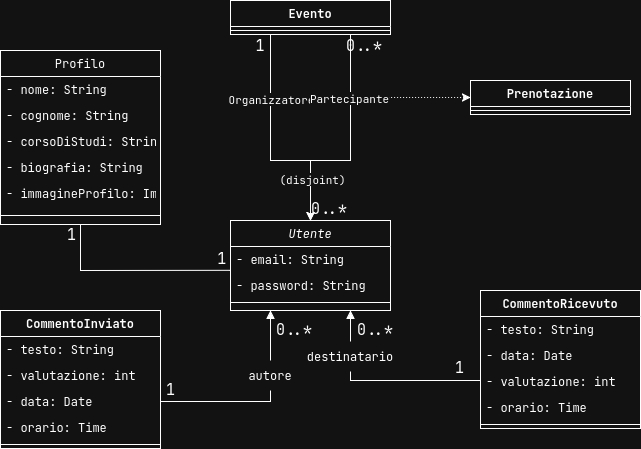
\includegraphics[width=\textwidth]{images/modello-del-dominio-profilo.png}
%\end{figure}

\subsection{Modello del dominio: Evento}
Il modello riguardante l'evento è presentato nel seguente diagramma.

%\begin{figure}[H]
%    \centering
%    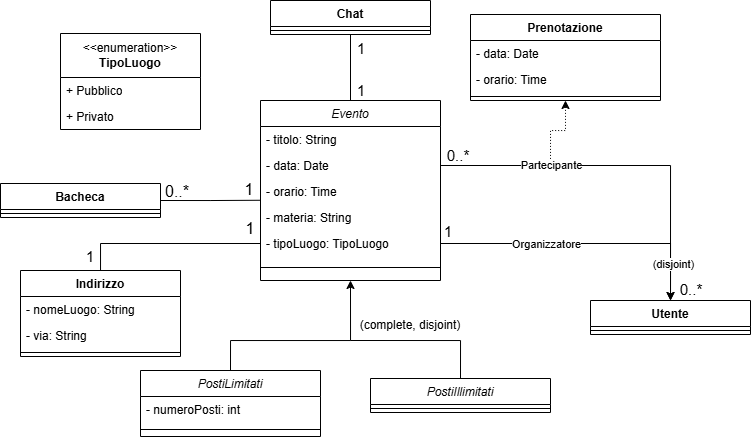
\includegraphics[width=\textwidth]{images/modello-del-dominio-evento.png}
%\end{figure}

\subsection{Modello del dominio: Filtro}
Il modello riguardante il filtro è presentato nel seguente diagramma.

%\begin{figure}[H]
%    \centering
%    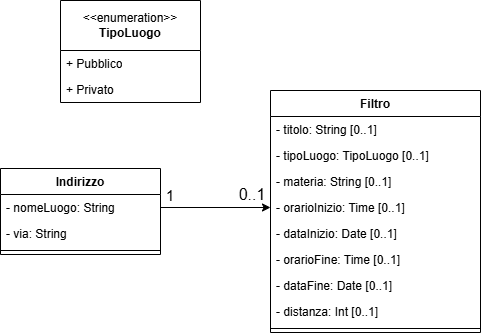
\includegraphics[width=\textwidth]{images/modello-del-dominio-filtro.png}
%\end{figure}

\subsection{Modello del dominio: Chat}
Il modello riguardante la chat è presentato nel seguente diagramma.

%\begin{figure}[H]
%    \centering
%    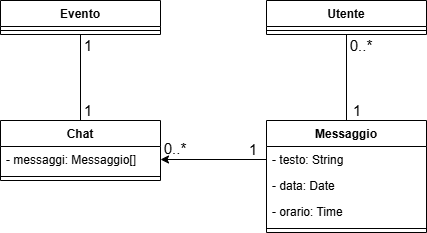
\includegraphics[width=\textwidth]{images/modello-del-dominio-chat.png}
%\end{figure}

\subsection{Modello del dominio: Commento}
Il modello riguardante il commento è presentato nel seguente diagramma.

%\begin{figure}[H]
%    \centering
%    \includegraphics[width=\textwidth]{images/modello-del-dominio-commento.png}
%\end{figure}

\subsection{Modello del dominio: Log}
Il modello riguardante il log è presentato nel seguente diagramma.

%\begin{figure}[H]
%    \centering
%    
\includegraphics[width=\textwidth]{images/modello-del-dominio-log.png}
%\end{figure}

% Architettura logica
\newpage
\section{Architettura logica}

\subsection{Struttura}

\subsection{Interazione}

\subsection{Comportamento}

% Piano di lavoro
\newpage
\section{Piano di lavoro}

\subsection{Caratteristiche primo prototipo (Giugno 2026)}

\subsection{Sviluppi futuri}

% Piano del collaudo
\newpage
\section{Piano del collaudo}

\subsection{Collaudo: Evento}

\subsection{Collaudo: Profilo}

% Progettazione
\newpage
\chapter{Progettazione}

% Progettazione architetturale
\section{Progettazione architetturale}

\subsection{Requisiti non funzionali}

\subsection{Scelta dell'architettura}

\subsection{Scelte tecnologiche}

\subsection{Diagramma dei package}

\subsection{Diagramma dei componenti}

% Progettazione di dettaglio
\newpage
\section{Progettazione di dettaglio}

\subsection{Struttura}

\subsection{Interazione}

\subsection{Interfacce utente}

% Progettazione della persistenza
\newpage
\section{Progettazione della persistenza}

% Progettazione del collaudo
\newpage
\section{Progettazione del collaudo}

\subsection{Test di unità: Evento}

\subsection{Test di unità: Profilo}

% Progettazione del deployment
\newpage
\section{Progettazione del deployment}

\subsection{Artefatti}

\subsection{Target di deploy}

% Di cosa parlare
\newpage
\section{Di cosa parlare}
\begin{itemize}[leftmargin=*]
    \item Pensare a se serve un amministratore
    \item per la creazione del log il prof dice di non metterlo da nessuna parte, guardare i best project. parla di 3 possibilità: 1) log viene analizzato manualmente da una persona al di fuori dell'applicazione (omino con scritto AS (l'attore) che si collega con freccia senza testa a cerchio con visualizzaLog in un'altra app) 2) uguale a quella di prima ma nell'applicazione stessa 3) algoritmo che in automatico si guarda il log e cerca cose strane. non c'è più visualizzaLog ma c'è analizzaLog (non la suggerisce, se vogliamo usare un algoritmo vuole che si faccia in un'altra applicazione)
    \item font da scegliere
\end{itemize}

% Errori
\section{Errori}
\begin{itemize}[leftmargin=*]
    \item 
\end{itemize}

% TODO
\section{TODO}
\begin{itemize}[leftmargin=*]
    \item togliere subsubsection dall'indice
    \item guardare le frecce e la sintassi in generale del modello del dominio
    \item capire se dividere anche nelle tabelle e in tutto il progetto (per esempio tabella informazioni / flusso) commento inviato/ricevuto o evento posti limitati / posti illimitati
\end{itemize}

\end{document}